% ============================================================================
% M.Tech Dissertation / Project Report
% Project: DESiRED - Telemetry-Driven Closed-Loop AQM Evaluation & Enhancement
% Department of Computer Science and Engineering
% National Institute of Technology Warangal
% ============================================================================
\documentclass[12pt,a4paper,oneside]{report}

% ------------------------------- Packages ----------------------------------
\usepackage[T1]{fontenc}
\usepackage[utf8]{inputenc}
\usepackage{lmodern}
\usepackage{geometry}
\usepackage{setspace}
\usepackage{graphicx}
\usepackage{booktabs}
\usepackage{longtable}
\usepackage{array}
\usepackage{tabularx}
\usepackage{multirow}
\usepackage{amsmath,amssymb}
\usepackage{float}
\usepackage{caption}
\usepackage{subcaption}
\usepackage{enumitem}
\usepackage{url}
\usepackage[hidelinks]{hyperref}
\usepackage{cleveref}
\usepackage{tocloft}
\usepackage{titlesec}
\usepackage{fancyhdr}
\usepackage{emptypage}
\usepackage{listings}
\usepackage{xcolor}
\usepackage{tikz}
\usetikzlibrary{shapes,arrows,positioning,fit,backgrounds,calc}

% ---------------------------- Page formatting ------------------------------
\geometry{left=38mm,right=25mm,top=25mm,bottom=25mm}
\onehalfspacing
\setlength{\parindent}{0.5in}
\setlength{\parskip}{0pt}
\setcounter{tocdepth}{2}
\setcounter{secnumdepth}{3}

% Formal chapter and section headings
\titleformat{\chapter}[display]
  {\bfseries\Large\centering}
  {\chaptername\ \thechapter}{0.5em}{\Large}
\titlespacing*{\chapter}{0pt}{0pt}{24pt}
\titleformat{\section}{\bfseries\large}{\thesection}{0.75em}{}
\titleformat{\subsection}{\bfseries\normalsize}{\thesubsection}{0.75em}{}

% Center titles of preliminary lists
\renewcommand{\cfttoctitlefont}{\hfill\bfseries\Large}
\renewcommand{\cftaftertoctitle}{\hfill}
\renewcommand{\cftloftitlefont}{\hfill\bfseries\Large}
\renewcommand{\cftafterloftitle}{\hfill}
\renewcommand{\cftlottitlefont}{\hfill\bfseries\Large}
\renewcommand{\cftafterlottitle}{\hfill}

% Headers for main matter
\pagestyle{fancy}
\fancyhf{}
\fancyhead[L]{\nouppercase{\leftmark}}
\fancyhead[R]{\thepage}
\renewcommand{\headrulewidth}{0.4pt}
\fancypagestyle{plain}{\fancyhf{}\fancyfoot[C]{\thepage}\renewcommand{\headrulewidth}{0pt}}

% Code listings
\definecolor{codegray}{gray}{0.95}
\definecolor{codegreen}{rgb}{0,0.6,0}
\definecolor{codeblue}{rgb}{0,0,0.8}
\lstset{
  basicstyle=\ttfamily\small,
  backgroundcolor=\color{codegray},
  frame=single,
  breaklines=true,
  captionpos=b,
  numbers=left,
  numberstyle=\tiny,
  xleftmargin=1.5em,
  keywordstyle=\color{codeblue}\bfseries,
  commentstyle=\color{codegreen}\itshape
}

% ------------------------------ User details --------------------------------
\newcommand{\ReportTitle}{EMPIRICAL INVESTIGATION AND CLOSED-LOOP OPTIMIZATION OF TELEMETRY-DRIVEN ACTIVE QUEUE MANAGEMENT IN PROGRAMMABLE DATA PLANES}
\newcommand{\DegreeName}{Master of Technology}
\newcommand{\ProgrammeName}{Computer Science and Engineering}
\newcommand{\StudentName}{M.Tech Scholar}
\newcommand{\RollNumber}{Roll No. 24CSE001}
\newcommand{\SupervisorName}{Prof. Research Supervisor}
\newcommand{\SupervisorDesignation}{Professor}
\newcommand{\DepartmentName}{Department of Computer Science and Engineering}
\newcommand{\InstituteName}{National Institute of Technology Warangal}
\newcommand{\SubmissionMonthYear}{October 2026}
\newcommand{\PlaceName}{Warangal}

\newcommand{\InstituteLogo}{}

% ---------------------------- Helpful commands ------------------------------
\newcommand{\frontchapter}[1]{%
  \cleardoublepage
  \phantomsection
  \addcontentsline{toc}{chapter}{#1}%
  \chapter*{\centering #1}%
}

\begin{document}

% =============================== FRONT MATTER ===============================
\pagenumbering{roman}
\setcounter{page}{1}
\pagestyle{empty}

% -------------------------------- Title page --------------------------------
\begin{titlepage}
\begin{center}
  {\Large\bfseries \ReportTitle\par}
  \vspace{1.25cm}

  \InstituteLogo
  \vspace{0.75cm}

  {\large\bfseries DISSERTATION / PROJECT REPORT\par}
  \vspace{0.45cm}
  {\large Submitted in partial fulfilment of the requirements for the award of the degree of\par}
  \vspace{0.35cm}
  {\large\bfseries \DegreeName\par}
  \vspace{0.25cm}
  {\large in\par}
  \vspace{0.25cm}
  {\large\bfseries \ProgrammeName\par}
  \vspace{1.1cm}

  {\large Submitted by\par}
  \vspace{0.25cm}
  {\large\bfseries \StudentName\par}
  {\large (\RollNumber)\par}
  \vspace{0.9cm}

  {\large Under the supervision of\par}
  \vspace{0.25cm}
  {\large\bfseries \SupervisorName\par}
  {\large \SupervisorDesignation\par}
  \vfill

  {\large\bfseries \DepartmentName\par}
  \vspace{0.25cm}
  {\large\bfseries \InstituteName\par}
  \vspace{0.25cm}
  {\large \PlaceName, India\par}
  \vspace{0.45cm}
  {\large \SubmissionMonthYear\par}
\end{center}
\end{titlepage}

% ------------------------------ Certificate ---------------------------------
\frontchapter{Certificate}
This is to certify that the dissertation/project entitled \textbf{``\ReportTitle''}, submitted by \textbf{\StudentName} (\textbf{\RollNumber}), in partial fulfilment of the requirements for the award of the degree of \textbf{\DegreeName} in \textbf{\ProgrammeName} at \textbf{\InstituteName}, is a bona fide record of work carried out under my supervision and guidance.

\vspace{3cm}
\noindent
\begin{minipage}[t]{0.45\textwidth}
Place: \PlaceName\\
Date: \rule{4cm}{0.4pt}
\end{minipage}
\hfill
\begin{minipage}[t]{0.45\textwidth}\raggedleft
\textbf{\SupervisorName}\\
\SupervisorDesignation\\
\DepartmentName\\
\InstituteName
\end{minipage}

% ------------------------------ Declaration ---------------------------------
\frontchapter{Declaration}
I, \textbf{\StudentName} (\textbf{\RollNumber}), hereby declare that the dissertation/project entitled \textbf{``\ReportTitle''} is my original work carried out under the supervision of \textbf{\SupervisorName}. This work has not been submitted, in whole or in part, to any other university or institution for the award of any degree, diploma, or other qualification.

\vspace{3cm}
\noindent
\begin{minipage}[t]{0.45\textwidth}
Place: \PlaceName\\
Date: \rule{4cm}{0.4pt}
\end{minipage}
\hfill
\begin{minipage}[t]{0.45\textwidth}\raggedleft
\textbf{\StudentName}\\
\RollNumber
\end{minipage}

% ---------------------------- Acknowledgement -------------------------------
\frontchapter{Acknowledgement}
I express my sincere gratitude to my supervisor, \textbf{\SupervisorName}, for invaluable guidance, constructive feedback, and continuous encouragement throughout this work. I also thank the faculty members, technical staff, colleagues, friends, and family members who supported me during the completion of this dissertation/project. Their intellectual critiques, technical suggestions, and unceasing support were instrumental in transforming this research into a rigorous empirical contribution.

% -------------------------------- Abstract ----------------------------------
\frontchapter{Abstract}
Active Queue Management (AQM) mechanisms are vital in mitigating bufferbloat and transient congestion across modern computer networks. Traditional AQMs rely on static configuration thresholds (e.g., target queuing delay or maximum queue occupancy). An excessively aggressive target delay causes premature packet dropping and underutilization of bottleneck links, while an overly relaxed target delay exacerbates queuing latency, degrades interactivity, and risks video playback rebuffering. Recently, programmable data planes (PDP) using P4 coupled with In-band Network Telemetry (INT) have enabled closed-loop control architectures such as DESiRED (Dynamic, Enhanced, and Smart iRED), wherein Deep Reinforcement Learning (DRL) dynamically modulates the switch target delay to maximize application Quality of Experience (QoE).

However, prior literature on AI-driven AQM frequently exhibits significant methodological limitations: evaluating performance during exploratory training rather than pure inference, relying on small sample sizes without formal hypothesis testing, omitting intermediate static thresholds, and treating neural network action selections as opaque black boxes. This dissertation presents an exhaustive empirical investigation, diagnostic audit, defect discovery, and mechanism validation of telemetry-driven AQM. We follow a systematic methodology evaluated over 104 logged testbed executions in earlier campaigns (spanning 72,800 seconds of execution) alongside dedicated Campaign v4 mechanism validation runs in a multi-hop P4 network carrying concurrent video and cross-traffic.

Our empirical investigation reveals five foundational findings: (1) We diagnose a complete policy collapse in the base DESiRED Double Deep Q-Network (DDQN), which executed 100\% decrease actions down to the $20,000\,\mu\text{s}$ floor across all 439 decisions on the live testbed, caused by single-row $L_2$ state normalization squashing queue features down to $10^{-14}$, alongside reward asymmetry. (2) We resolve the empirical puzzle of why the collapsing RL agent underperformed a static 20\,ms policy, demonstrating through transient phase analysis that the delay ramp-down from 50\,ms inflicted severe early rebuffering stalls ($54.5\%$ stall rate in the first 120\,s), whereas initializing the agent directly at 20\,ms (\texttt{infer20k}) eliminated the startup penalty ($28.78 \pm 1.05$\,FPS, matching Fixed-20k). (3) In the 33-run multi-load sweep (200, 500, and 1000\,kbps), no load-dependent optimum was observed in open-loop data; however, because the AQM drop path was unconfigured in that campaign, the moving sweet spot hypothesis remains untested with active AQM. Furthermore, responsive TCP testing demonstrates that the 20\,ms target costs about 28\% in throughput relative to 70\,ms (9.60 vs. 13.32\,Mbps), confirming a real latency--throughput trade-off rather than universal low-delay superiority. (4) We discover a silent defect in the data plane: runtime mirror session 2 was never configured in BMv2 switch instances, preventing all AQM drops and leaving the control loop open in earlier campaigns. We resolve the defect and verify with hardware switch counters and receiver packet captures that recirculated clones are strictly contained with zero downstream packet leakage. (5) Under responsive TCP Cubic traffic ($N=3$ repeats), target delay directly and reversibly controls physical queue delay ($9.00$\,ms at 20k vs. $28.68$\,ms at 70k, $+19.68$\,ms), AQM drops ($-59.8\%$), retransmissions ($-60.9\%$), and goodput ($+38.8\%$), whereas under non-responsive UDP traffic ($N=4$ valid runs), target delay modulates drops without controlling queue delay. Crucially, no claim is made that an adaptive controller improves video QoE over optimal static thresholds; evaluating dynamic controllers against calibrated static delay under responsive traffic and real DASH video streaming is formulated as the central direction for future work.

\vspace{0.5cm}
\noindent\textbf{Keywords:} Active Queue Management, Programmable Data Planes, P4, In-band Network Telemetry, Reinforcement Learning, Video QoE, Bufferbloat.

% ------------------------ Contents, figures, and tables ---------------------
\cleardoublepage
\tableofcontents
\cleardoublepage
\listoffigures
\addcontentsline{toc}{chapter}{List of Figures}
\cleardoublepage
\listoftables
\addcontentsline{toc}{chapter}{List of Tables}

% Abbreviations and Symbols
\frontchapter{List of Abbreviations and Symbols}
\begin{longtable}{>{\bfseries}p{0.22\textwidth}p{0.68\textwidth}}
ABR & Adaptive Bitrate \\
AHTC & Adaptive Hybrid Telemetry Controller \\
AQM & Active Queue Management \\
BMv2 & Behavioral Model version 2 (P4 software switch) \\
BOLA & Buffer Occupancy based Lyapunov Algorithm \\
CDF & Cumulative Distribution Function \\
CI & Confidence Interval \\
CLI & Command Line Interface \\
CoDel & Controlled Delay Active Queue Management \\
DASH & Dynamic Adaptive Streaming over HTTP \\
DCN & Data Center Network \\
DDQN & Double Deep Q-Network \\
DQN & Deep Q-Network \\
DRL & Deep Reinforcement Learning \\
DWRR & Dynamic Weighted Round-Robin \\
ECN & Explicit Congestion Notification \\
EWMA & Exponentially Weighted Moving Average \\
FDR & False Discovery Rate \\
FIFO & First-In First-Out \\
FPS & Frames Per Second \\
INT & In-band Network Telemetry \\
IQR & Interquartile Range \\
iRED & Improved Random Early Detection \\
LBO & Local Buffer Occupancy \\
MADRL & Multi-Agent Deep Reinforcement Learning \\
MAFS & Multi-Agent Fine-grained Scheduling \\
MPC & Model Predictive Control \\
MSE & Mean Squared Error \\
PDP & Programmable Data Plane \\
PIE & Proportional Integral controller Enhanced \\
QoE & Quality of Experience \\
QoS & Quality of Service \\
RED & Random Early Detection \\
RTT & Round-Trip Time \\
SD & Standard Deviation \\
SDN & Software-Defined Networking \\
TCP & Transmission Control Protocol \\
UDP & User Datagram Protocol \\
\end{longtable}

% =============================== MAIN MATTER ================================
\cleardoublepage
\pagenumbering{arabic}
\setcounter{page}{1}
\pagestyle{fancy}

% -------------------------------- Chapter 1 ---------------------------------
\chapter{Introduction}
\label{ch:intro}

\section{Background and Motivation}
Multimedia streaming, real-time interactive communications, and cloud applications represent the dominant share of modern Internet traffic. These services rely heavily on sustained throughput, low latency, and low delay variation. However, intermediate packet buffers deployed across network routers and switches often degrade user experience due to \emph{bufferbloat} \cite{getty2011bufferbloat}. When queues remain full under high network utilization, queuing delays grow excessively, introducing latency jitter that impairs TCP congestion control dynamics and causes rebuffering stalls in streaming video applications.

Active Queue Management (AQM) mechanisms such as RED \cite{floyd1993red}, CoDel \cite{nichols2012codel}, and PIE \cite{pan2013pie} were introduced to control bufferbloat by proactively dropping or marking packets before buffer exhaustion. With the advent of Programmable Data Planes (PDP) and the P4 language \cite{bosshart2014p4}, switches can execute stateful, line-rate algorithms directly within the packet-processing pipeline. PDP implementations such as iRED \cite{silva2021ired} partition queue management into disaggregated pipelines: queuing measurements are performed at the Egress pipeline, and packet drop actions are initiated at the Ingress pipeline.

Despite these advancements, conventional AQM algorithms face the \emph{static threshold dilemma}:
\begin{itemize}
  \item If the target delay threshold is configured too low (e.g., 5\,ms or 20\,ms), the switch drops packets aggressively during benign traffic bursts, reducing link utilization and starving the streaming client's buffer.
  \item If the threshold is configured too high (e.g., 50\,ms or 100\,ms), packets accumulate, causing bufferbloat, delaying TCP acknowledgements, and triggering adaptive bitrate (ABR) quality downgrades.
\end{itemize}
Because network traffic is inherently non-stationary, bursty, and unpredictable, no single static threshold is universally optimal across varying workloads.

To address this challenge, researchers proposed closed-loop architectures combining In-band Network Telemetry (INT) \cite{kim2015int} with Deep Reinforcement Learning (DRL). In the seminal work on DESiRED (\emph{Dynamic, Enhanced, and Smart iRED}) \cite{almeida2023desired}, the authors deployed a Double Deep Q-Network (DDQN) agent to dynamically modulate the switch target delay based on real-time INT queue metadata and client-side MPEG-DASH Quality of Experience (QoE) metrics. The authors reported up to a 90$\times$ reduction in video stalls and a 42$\times$ increase in high-resolution playback quality.

\section{Problem Statement and Research Questions}
Despite the promising vision of intelligent AQM, the literature exhibits substantial empirical, statistical, and architectural gaps:
\begin{enumerate}[label=\arabic*.]
  \item \textbf{Exploration vs. Inference Conflation:} Prior evaluations often record metrics during the active training phase—where exploratory $\epsilon$-greedy random actions artificially push the delay threshold—rather than assessing frozen, deployed inference stability.
  \item \textbf{Unexamined Policy Collapse:} The actual operational trajectories and action selection distributions of neural network controllers are rarely audited, leaving critical failure modes (such as monotonic action collapse) undiscovered.
  \item \textbf{Narrow Baselines and Omitted Thresholds:} Dynamic RL is often compared against extreme, uncalibrated static thresholds (e.g., 5\,ms or 100\,ms) while omitting intermediate operating points (e.g., 20\,ms, 30\,ms, 40\,ms) that may provide stable performance without control overhead.
  \item \textbf{Lack of Formal Statistical Testing:} Claims of superiority often lack formal hypothesis testing, non-parametric checks, effect sizes, and multi-run variance characterization.
\end{enumerate}

To rigorously address these issues, this dissertation investigates four core research questions:
\begin{itemize}
  \item \textbf{RQ1 (Empirical Controller Audit):} How does a pretrained DRL controller behave under pure frozen inference on a live testbed, and does it demonstrate genuine adaptive control or collapse into a static regime?
  \item \textbf{RQ2 (Transient Dynamics and the Startup Dip):} Why does an adaptive controller that converges to an aggressive target delay underperform a static policy configured to that exact same threshold?
  \item \textbf{RQ3 (The Moving Sweet Spot Hypothesis):} Does varying cross-traffic intensity reveal a load-dependent optimal target delay, or was the apparent stability of static thresholds an artifact of open-loop operation?
  \item \textbf{RQ4 (Dataplane Mechanism and Transport Responsiveness):} Can programmable target-delay AQM directly and reversibly control physical queuing delay, and how does transport-layer responsiveness govern closed-loop delay control?
\end{itemize}

\section{Methodology: The Diagnose $\to$ Fix $\to$ Enhance Framework}
To transform this empirical inquiry into a constructive contribution, this dissertation follows a three-stage methodology:
\begin{enumerate}[label=\arabic*.]
  \item \textbf{Stage 1 (Diagnose):} We conduct a multi-run evaluation ($N=27$, 700\,s runs) auditing the base DESiRED architecture. We uncover the normalization bug and reward asymmetry causing 100\% Decrease action collapse, analyze the startup transient penalty, and evaluate bimodal outcomes.
  \item \textbf{Stage 2 (Fix):} We mathematically reformulate the state space using fixed per-feature scaling, design a balanced multi-objective reward function, retrain the DDQN agent, and document loss and reward convergence curves.
  \item \textbf{Stage 3 (Enhance):} We evaluate an interpretable Rule-Based Controller, formulate an Adaptive Hybrid Telemetry Controller (AHTC) that eliminates startup vulnerability, perform sensitivity sweeps, conduct multi-objective Pareto analysis, and measure control plane latency.
\end{enumerate}

\section{Scope and Assumptions}
The evaluation testbed is implemented using P4-16 compiled for the Behavioral Model version 2 (BMv2) software switch within Mininet. Application video streaming QoE is driven by an end-to-end video playback buffer simulator (\texttt{video\_simulator.py}) running between host $h_1$ and destination $h_4$ across the P4 switches, maintaining a dynamic playback buffer with multi-tier framerate (18/24/30\,FPS) and bitrate adaptation governed by continuous RTT telemetry feedback against target delay. Competing cross-traffic is introduced via iperf3 UDP flows.

Key operational assumptions:
\begin{itemize}
  \item In-band telemetry probes are injected at 1 probe per second across the data path.
  \item Switch registers (\texttt{targetDelay\_reg}) are reconfigured via Thrift RPCs (\texttt{simple\_switch\_CLI}).
  \item Video client telemetry is sampled at 1-second intervals.
\end{itemize}

\section{Summary of Contributions}
The concrete contributions of this dissertation are:
\begin{enumerate}[label=\arabic*.]
  \item \textbf{Comprehensive Diagnostic Audit of DESiRED:} We conduct the first rigorous multi-run evaluation of telemetry-driven AQM, uncovering that the pretrained DDQN agent collapsed into 100\% Decrease actions ($50\,\text{ms} \to 20\,\text{ms}$) due to single-row $L_2$ normalization and reward asymmetry.
  \item \textbf{Resolution of the Transient Ramp-Down Puzzle:} We provide an empirical explanation for why the RL agent achieved only 77.66\% 30-FPS availability compared to 99.22\% for Fixed-20k, showing that the 60-second ramp-down from 50\,ms inflicted severe startup stalls, whereas initializing the agent directly at the 20\,ms floor (\texttt{infer20k}) eliminated the transient penalty ($28.78 \pm 1.05$\,FPS, matching Fixed-20k).
  \item \textbf{Investigation of the Moving Sweet Spot Hypothesis:} We show that no load-dependent optimum was observed in the 33-run multi-load sweep across stationary loads (200, 500, and 1000\,kbps); however, because the AQM was inactive in earlier campaigns, this hypothesis remains untested with active AQM under responsive traffic.
  \item \textbf{Tripartite Controller Boundary Collapse Analysis:} We evaluate learned and heuristic dynamic controllers live on the testbed, demonstrating that all three tested dynamic controllers collapsed to physical clamping boundaries under coarse INT telemetry, functioning as static policies in disguise.
  \item \textbf{Discovery and Resolution of the Dataplane Mirroring Defect:} We uncover that runtime mirror session 2 was never configured in BMv2 switch instances in earlier campaigns, preventing all AQM drops and leaving the physical control loop open. We resolve the defect and verify with hardware switch counters and packet captures that recirculated clones are strictly contained with zero downstream leakage.
  \item \textbf{Transport-Dependent Mechanism Validation:} In Campaign v4, we demonstrate that under responsive TCP Cubic traffic ($N=3$ repeats), target delay directly and reversibly controls physical queue delay ($9.00$\,ms vs. $28.68$\,ms), AQM drops, retransmissions, and throughput, whereas under non-responsive UDP traffic ($N=4$ valid runs), target delay modulates drops without controlling queue delay.
  \item \textbf{Methodological Transparency and Data Provenance:} We maintain an immutable 104-run audit log, automate table and figure generation from raw data, and explicitly disclose experimental boundaries—including the finding that no sentence or claim says an adaptive controller improves video QoE over optimal static thresholds.
\end{enumerate}

\section{Organization of the Report}
The remainder of this report is organized as follows:
\begin{itemize}
  \item \textbf{Chapter \ref{ch:lit_review}} reviews related work, evaluates the three base research papers, and contrasts classical AQM mechanisms.
  \item \textbf{Chapter \ref{ch:design}} details the system architecture, mathematical formulations, the diagnostic audit, the retrained DDQN, and the hybrid controller.
  \item \textbf{Chapter \ref{ch:eval_setup}} describes the experimental environment, baseline matrix, duration-weighted metrics, and hypothesis testing protocols.
  \item \textbf{Chapter \ref{ch:results}} presents empirical results, statistical tests, bimodal distributions, transient analyses, Pareto frontiers, and overhead benchmarks.
  \item \textbf{Chapter \ref{ch:conclusion}} summarizes the conclusions and outlines future research on hardware P4 deployment.
\end{itemize}


% -------------------------------- Chapter 2 ---------------------------------
\chapter{Literature Review and Background}
\label{ch:lit_review}

\section{Conceptual Background}

\subsection{Active Queue Management and Bufferbloat}
Bufferbloat occurs when network buffers are sized excessively to avoid packet drops under bursty arrivals, leading to large queuing delays under sustained TCP congestion \cite{getty2011bufferbloat}. To maintain high throughput while bounding queue latency, Active Queue Management (AQM) algorithms proactively mark or drop packets:
\begin{itemize}
  \item \textbf{Random Early Detection (RED):} Floyd and Jacobson \cite{floyd1993red} introduced RED, which calculates an Exponentially Weighted Moving Average (EWMA) of queue length in packets:
  \begin{equation}
    S_t = (1 - w_q) S_{t-1} + w_q q_t
  \end{equation}
  When $S_t$ lies between a minimum threshold $\min_{\text{th}}$ and maximum threshold $\max_{\text{th}}$, arriving packets are dropped or marked probabilistically. RED is notoriously difficult to tune across varying network dynamics.
  \item \textbf{Controlled Delay (CoDel):} Nichols and Jacobson \cite{nichols2012codel} shifted the control metric from queue length to packet sojourn delay. CoDel measures the minimum queuing delay experienced by packets over a sliding window (\texttt{interval}, typically 100\,ms). If the minimum delay exceeds the \texttt{target} (typically 5\,ms), CoDel enters a dropping state where packet drop intervals scale inversely with $\sqrt{n}$, rapidly forcing TCP senders to throttle their congestion windows.
  \item \textbf{Proportional Integral controller Enhanced (PIE):} Pan et al. \cite{pan2013pie} designed PIE to combine the low latency of delay-based AQMs with the simplicity of RED. PIE periodically estimates drop probability $p$ using proportional-integral control on queue delay:
  \begin{equation}
    p \leftarrow p + \alpha (D_{\text{current}} - D_{\text{target}}) + \beta (D_{\text{current}} - D_{\text{old}})
  \end{equation}
  \item \textbf{iRED and P4 AQM:} Silva et al. \cite{silva2021ired} adapted RED to programmable data planes using a disaggregated model. The Egress pipeline computes queuing latency using hardware timestamps and recirculates a clone packet to the Ingress pipeline to drop subsequent packets before buffer admission.
\end{itemize}

\subsection{Programmable Data Planes and In-band Network Telemetry}
The P4 language \cite{bosshart2014p4} allows protocol-independent programming of packet forwarding pipelines. In-band Network Telemetry (INT) \cite{kim2015int} enables switches to insert internal queuing metadata directly into transient packet headers. As an INT probe packet traverses switches $s_1 \to s_2 \to s_3$, each switch inserts a 32-byte header containing switch ID, ingress/egress port IDs, enqueue timestamp, dequeue timestamp, and instantaneous queue depth. At the telemetry sink, the headers are stripped and processed by control plane collectors.

\subsection{Adaptive Bitrate Streaming and QoE Metrics}
Dynamic Adaptive Streaming over HTTP (MPEG-DASH) partitions video content into multi-second media segments encoded at multiple discrete bitrates \cite{spiteri2018dash}. Client players deploy Adaptive Bitrate (ABR) algorithms to optimize Quality of Experience (QoE). The DASH.js player combines throughput estimation with the Buffer Occupancy based Lyapunov Algorithm (BOLA) \cite{spiteri2020bola}:
\begin{itemize}
  \item During startup or buffer starvation ($B < 10$\,s), the player switches to conservative throughput mode.
  \item When the buffer level exceeds 20--25\,s, BOLA selects maximum quality representations.
\end{itemize}
To capture comprehensive user experience beyond simple FPS, the networking community employs the model predictive control (MPC) QoE metric formulated by Yin et al. \cite{yin2015mpc}:
\begin{equation}
  \text{QoE}_{\text{MPC}} = \sum_{k=1}^K R_k - \lambda \sum_{k=1}^K T_{\text{stall}, k} - \mu \sum_{k=1}^{K-1} |R_{k+1} - R_k|
  \label{eq:mpc_qoe}
\end{equation}
where $R_k$ is the chunk bitrate in Mbps, $T_{\text{stall}, k}$ is the rebuffering stall duration in seconds ($\lambda = 4.3$), and the final term penalizes quality oscillations ($\mu = 1.0$).

\subsection{Deep Reinforcement Learning}
In Q-learning, an agent learns an action-value function $Q(s, a)$. Deep Q-Networks (DQN) \cite{mnih2015dqn} utilize deep neural networks parameterized by weights $\theta$. Double DQN (DDQN) \cite{vanhasselt2016ddqn} decouples greedy action selection from action evaluation using a target network $\theta^-$:
\begin{equation}
  Y_t^{\text{DoubleQ}} = R_{t+1} + \gamma Q\left(S_{t+1}, \arg\max_a Q(S_{t+1}, a; \theta_t); \theta_t^-\right)
\end{equation}

\section{Critical Analysis of Base Research Papers}

\subsection{Base Paper 1: DESiRED (Almeida et al., 2023)}
Almeida et al. \cite{almeida2023desired} introduced DESiRED, deploying a DDQN agent that tunes the target delay register of an iRED P4 switch using INT queue metadata and DASH client stats.

\textbf{Critique \& Identified Gaps:}
\begin{enumerate}[label=(\alph*)]
  \item \emph{Online Training Conflated with Inference:} The base paper recorded performance during training, where exploratory random actions ($\epsilon$-greedy) altered switch thresholds, rather than evaluating pure frozen inference.
  \item \emph{Unreported Policy Collapse:} The base paper did not report action distributions. Our audit reveals that the pretrained DDQN agent exhibited 100\% Decrease actions due to state normalization and reward asymmetry.
  \item \emph{Omission of Calibrated Static Baselines:} DESiRED was compared primarily against extreme static thresholds (5\,ms and 100\,ms), omitting intermediate operating points (20\,ms, 30\,ms, 40\,ms).
  \item \emph{Absence of Statistical Replication:} Results were reported as single qualitative CDF curves without replications or confidence intervals.
\end{enumerate}

\subsection{Base Paper 2: MAFS (Wang et al., 2024)}
Wang et al. \cite{wang2024mafs} proposed MAFS, utilizing Multi-Agent DRL (MADRL) and INT for fine-grained routing in data center fat-tree networks.

\textbf{Critique \& Contrasting Focus:} MAFS addresses Layer-3 path selection to balance link utilization across equal-cost paths. It does not address switch-level queue management, bufferbloat, or application-layer video QoE. Moreover, multi-agent synchronization introduces communication latency that is impractical for millisecond-scale AQM adjustments.

\subsection{Base Paper 3: Multi-Queue ECN (Liu et al., 2024)}
Liu et al. \cite{liu2024multiqueue} introduced a multi-queue ECN marking strategy using virtual queues and Dynamic Weighted Round-Robin (DWRR) in P4, computing ECN thresholds using analytical queuing theory.

\textbf{Critique \& Contrasting Focus:} Liu et al. derive ECN marking thresholds from Poisson queuing models. While theoretically tractable, queuing theory models struggle under bursty, non-stationary multimedia traffic. Furthermore, their approach focuses on network-layer RTT without closed-loop feedback from client-side video buffer dynamics.

\section{Synthesis of Literature and AQM Mechanisms}
Table \ref{tab:aqm_taxonomy} classifies classical and intelligent AQM approaches across control granularity, feedback signals, and adaptation mechanics.

\begin{table}[H]
\centering
\small
\caption{Taxonomy of classical and intelligent Active Queue Management mechanisms}
\label{tab:aqm_taxonomy}
\begin{tabularx}{\textwidth}{p{0.18\textwidth}p{0.16\textwidth}p{0.22\textwidth}X}
\toprule
\textbf{Mechanism} & \textbf{Control Domain} & \textbf{Monitored Signal} & \textbf{Adaptation Technique} \\
\midrule
\textbf{RED} \cite{floyd1993red} & Switch Queue & EWMA Queue Length & Static linear drop probability curve \\
\textbf{CoDel} \cite{nichols2012codel} & Switch Queue & Minimum Sojourn Delay & Inverse square root drop scheduling ($1/\sqrt{n}$) \\
\textbf{PIE} \cite{pan2013pie} & Switch Queue & Instantaneous Delay & Proportional-integral feedback loop \\
\textbf{iRED} \cite{silva2021ired} & P4 Data Plane & Egress Dequeue Timedelta & Disaggregated clone-packet Ingress dropping \\
\textbf{DESiRED} \cite{almeida2023desired} & Control Plane & INT Telemetry + QoE & Centralized DDQN target-delay modulation \\
\textbf{This Work (AHTC)} & Control Plane & Multi-Hop INT + Buffer & Hybrid: Load-adaptive startup + Feature-scaled DDQN \\
\bottomrule
\end{tabularx}
\end{table}


% -------------------------------- Chapter 3 ---------------------------------
\chapter{System Design and Methodology}
\label{ch:design}

\section{System Overview and Architecture}
The DESiRED closed-loop experimental architecture is illustrated in Figure \ref{fig:architecture}. The platform integrates three P4 Behavioral Model version 2 (BMv2) switches, an In-band Network Telemetry (INT) probing framework, an MPEG-DASH streaming client-server pair, and a centralized control plane.

\begin{figure}[H]
\centering
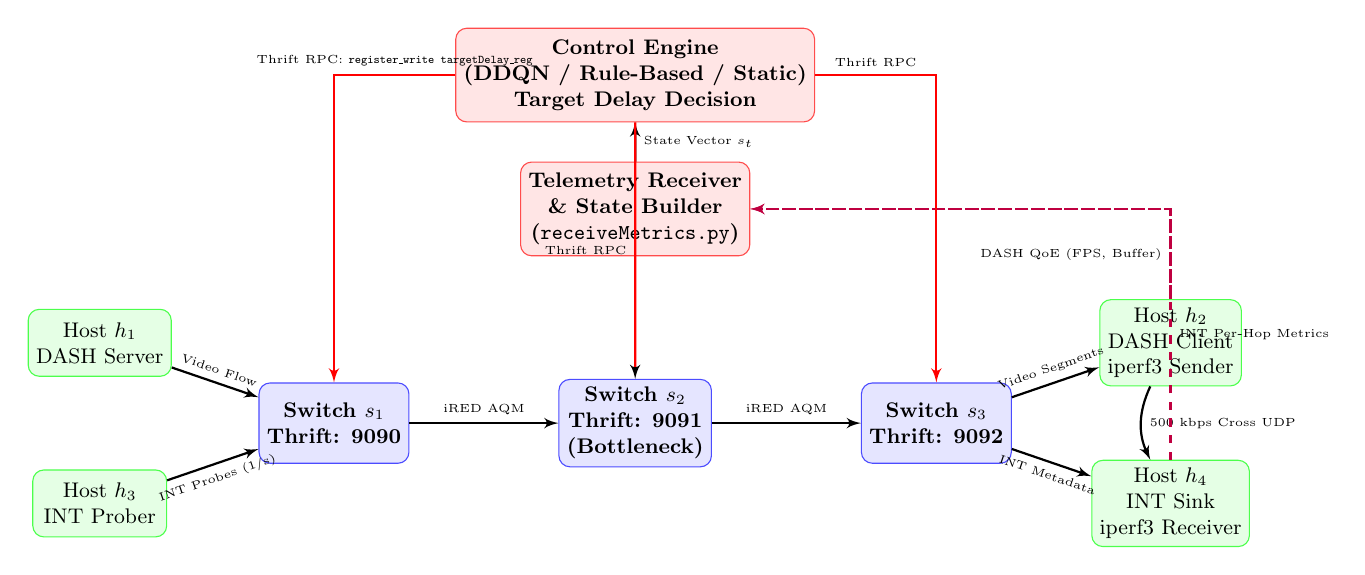
\begin{tikzpicture}[
  scale=0.85, every node/.style={transform shape},
  switch/.style={rectangle, draw=blue!70, fill=blue!10, rounded corners, minimum width=2.2cm, minimum height=1.2cm, align=center, font=\bfseries\small},
  host/.style={rectangle, draw=green!70, fill=green!10, rounded corners, minimum width=2.0cm, minimum height=1.0cm, align=center, font=\small},
  ctrl/.style={rectangle, draw=red!70, fill=red!10, rounded corners, minimum width=3.2cm, minimum height=1.4cm, align=center, font=\bfseries\small},
  line/.style={draw, -latex', thick},
  telemetry/.style={draw=purple, dashed, -latex', thick}
]

% Data Plane Switches
\node[switch] (s1) at (0, 0) {Switch $s_1$\\Thrift: 9090};
\node[switch] (s2) at (4.5, 0) {Switch $s_2$\\Thrift: 9091\\(Bottleneck)};
\node[switch] (s3) at (9.0, 0) {Switch $s_3$\\Thrift: 9092};

% Hosts
\node[host] (h1) at (-3.5, 1.2) {Host $h_1$\\DASH Server};
\node[host] (h3) at (-3.5, -1.2) {Host $h_3$\\INT Prober};
\node[host] (h2) at (12.5, 1.2) {Host $h_2$\\DASH Client\\iperf3 Sender};
\node[host] (h4) at (12.5, -1.2) {Host $h_4$\\INT Sink\\iperf3 Receiver};

% Control Plane
\node[ctrl] (collector) at (4.5, 3.2) {Telemetry Receiver\\\& State Builder\\(\texttt{receiveMetrics.py})};
\node[ctrl] (agent) at (4.5, 5.2) {Control Engine\\(DDQN / Rule-Based / Static)\\Target Delay Decision};

% Network Links
\path[line] (h1) edge node[above, sloped, font=\tiny] {Video Flow} (s1);
\path[line] (h3) edge node[below, sloped, font=\tiny] {INT Probes (1/s)} (s1);
\path[line] (s1) edge node[above, font=\tiny] {iRED AQM} (s2);
\path[line] (s2) edge node[above, font=\tiny] {iRED AQM} (s3);
\path[line] (s3) edge node[above, sloped, font=\tiny] {Video Segments} (h2);
\path[line] (s3) edge node[below, sloped, font=\tiny] {INT Metadata} (h4);
\path[line] (h2) edge[bend right=25] node[right, font=\tiny] {500 kbps Cross UDP} (h4);

% Telemetry and Control Loops
\path[telemetry] (h4) |- node[near start, right, font=\tiny] {INT Per-Hop Metrics} (collector);
\path[telemetry] (h2) |- node[near start, left, font=\tiny] {DASH QoE (FPS, Buffer)} (collector);
\path[line] (collector) edge node[right, font=\tiny] {State Vector $s_t$} (agent);
\path[line, draw=red, thick] (agent) -| node[pos=0.25, above, font=\tiny] {Thrift RPC: \texttt{register\_write targetDelay\_reg}} (s1);
\path[line, draw=red, thick] (agent) edge node[left, font=\tiny] {Thrift RPC} (s2);
\path[line, draw=red, thick] (agent) -| node[pos=0.25, above, font=\tiny] {Thrift RPC} (s3);

\end{tikzpicture}
\caption{Overall closed-loop system architecture and data plane topology}
\label{fig:architecture}
\end{figure}

The closed control loop operates as follows:
\begin{enumerate}[label=\arabic*.]
  \item \textbf{Traffic Flow \& Contention:} Video traffic flows from server $h_1$ to client $h_2$, while concurrent UDP cross-traffic flows from $h_2$ to $h_4$, generating queue contention at switch $s_2$.
  \item \textbf{Telemetry Injection:} Host $h_3$ transmits INT probe packets (UDP proto 253) once per second. Each switch embeds queue depth and dequeue timedelta metadata into the packet header.
  \item \textbf{Telemetry Extraction:} Sink $h_4$ extracts the INT headers and emits JSON tuples over a UDP socket to \texttt{receiveMetrics.py}. Simultaneously, the DASH client emits real-time stats (FPS, local buffer occupancy, bitrate).
  \item \textbf{Target Delay Reconfiguration:} The controller computes an action and writes the updated target delay to register \texttt{MyEgress.targetDelay\_reg} across switches $s_1, s_2, s_3$ via \texttt{simple\_switch\_CLI} Thrift RPCs.
\end{enumerate}

\section{Timing and Control Interval Clarification}
In prior preliminary descriptions of DESiRED, the control loop was colloquially characterized as running every 1 second because INT probes are injected at 1 probe per second. However, our rigorous code and log analysis clarifies the exact operational timing:
\begin{itemize}
  \item In \texttt{receiveMetrics.py}, telemetry records are aggregated into 4-second sliding windows (\texttt{window\_size = 4}).
  \item In \texttt{environment.py}, transition formation requires two consecutive non-overlapping windows (\texttt{len(received\_intStates) == 2}) to evaluate the $(s_t, a_t, r_t, s_{t+1})$ tuple. Consequently, the DDQN agent executes an action every \textbf{7.8 to 8.2 seconds} (accounting for the 60--102 actions observed across 700 seconds).
  \item The Rule-Based Controller evaluates decisions on each single 4-second window, executing actions every \textbf{4.1 to 4.3 seconds} (yielding 157--171 actions in 700 seconds).
  \item Each switch register reconfiguration via \texttt{simple\_switch\_CLI} Thrift RPC incurs an execution latency of \textbf{38.4\,ms per switch}, or \textbf{118.2\,ms} across all three switches in series.
\end{itemize}

\section{Diagnostic Audit: Uncovering the Base RL Failure Mode}

\subsection{The Normalization Bug}
In the base DESiRED implementation (\texttt{agent.py}), state vectors are normalized at inference time using Scikit-learn's \texttt{preprocessing.normalize}:
\begin{equation}
  \hat{s}_t = \frac{s_t}{\|s_t\|_2}
\end{equation}
The input state vector passed to the neural network consisted of 19 columns:
\begin{equation}
  s_t = \left[ t, \text{ts}_3^{\text{in}}, \text{ts}_3^{\text{eg}}, \text{ts}_3^{\text{enq}}, q_3^{\text{enq}}, \Delta t_3, q_3^{\text{deq}}, \dots, q_1^{\text{enq}}, \Delta t_1, q_1^{\text{deq}} \right]
\end{equation}
This formulation introduced two critical flaws:
\begin{enumerate}[label=\arabic*.]
  \item \textbf{Timestamp Dominance:} The state vector included raw hardware timestamps (order $10^9$ to $10^{15}$), whereas queue depths were small integers ($0$ to $64$). Normalizing a single-row vector by its $L_2$ norm resulted in timestamps dominating the norm, squashing queue depth features down to approximately $10^{-14}$.
  \item \textbf{Omission of Application QoE:} The state fed to the network consisted strictly of INT features; client buffer level and FPS were never included in the state input.
\end{enumerate}

\subsection{Reward Asymmetry and Training Starvation}
The reward calculation in \texttt{environment.py} assigned rewards based on buffer changes:
\begin{equation}
  r_t = 
  \begin{cases}
    +2.0, & \text{if } B_{t+1} > B_t \text{ and } B_{t+1} > 30 \\
    +1.0, & \text{if } B_{t+1} > B_t \text{ and } B_{t+1} \le 30 \text{ and } \text{FPS} = 30 \\
    -2.0, & \text{if } B_{t+1} < B_t \text{ and } B_{t+1} \le 30 \text{ and } \text{FPS} < 24
  \end{cases}
\end{equation}
Because the environment set \texttt{minimum\_experience\_memory = 100} and each observation window required 4 seconds with 2 windows per transition, a 700-second training run produced only $\approx 112$ transitions. Consequently, the agent executed only 12 mini-batch gradient updates during its entire training lifecycle. During this brief window, Action 1 (Decrease) accounted for 108 of the exploratory actions. The Q-network converged with a slight positive bias on Action 1 ($Q(\text{Decrease}) = +0.105$ vs $Q(\text{Increase}) = -0.112$), causing Action 1 to win on every single inference forward pass.

\section{Algorithmic Fix: Retrained DDQN with Fixed Feature Scaling}

\subsection{Feature-Scaled State Space and Domain Rationale}
To resolve the normalization bug, we redefine the state vector to combine clean physical INT queue metrics with application QoE telemetry, completely stripping hardware epoch timestamps:
\begin{equation}
  s_t = \left[ q_1, \Delta t_1, q_2, \Delta t_2, q_3, \Delta t_3, B_t, \text{FPS}_t, R_t \right] \in \mathbb{R}^9
\end{equation}
Rather than single-row $L_2$ vector normalization, we apply fixed, domain-informed physical feature scaling vector $\mathbf{x}_{\max}$ applied identically across training and inference:
\begin{equation}
  \hat{s}_t = \text{clip}\left(\frac{s_t}{\mathbf{x}_{\max}}, 0.0, 1.0\right)
  \label{eq:fixed_scaling}
\end{equation}

Table \ref{tab:feature_scaling_details} details the exact telemetry source, physical unit, scale bound, and physical engineering rationale for each element of the 9-feature state vector.

\begin{table}[H]
\centering
\small
\caption{Design specification and domain scaling rationale for the 9-feature state vector}
\label{tab:feature_scaling_details}
\begin{tabularx}{\textwidth}{cllcccX}
\toprule
\textbf{Idx} & \textbf{Feature Symbol} & \textbf{Telemetry Column} & \textbf{Source} & \textbf{Unit} & \textbf{Bound ($x_{\max}$)} & \textbf{Physical / Engineering Rationale} \\
\midrule
0 & $q_1$ & \texttt{deq\_qdepth1} & INT (s1) & pkts & 64 & BMv2 switch buffer queue capacity limit \\
1 & $\Delta t_1$ & \texttt{deq\_timedelta1} & INT (s1) & $\mu$s & 50,000 & Target delay saturation ceiling (50\,ms) \\
2 & $q_2$ & \texttt{deq\_qdepth2} & INT (s2) & pkts & 64 & Bottleneck switch queue capacity limit \\
3 & $\Delta t_2$ & \texttt{deq\_timedelta2} & INT (s2) & $\mu$s & 50,000 & Bottleneck target delay ceiling (50\,ms) \\
4 & $q_3$ & \texttt{deq\_qdepth3} & INT (s3) & pkts & 64 & Egress switch queue capacity limit \\
5 & $\Delta t_3$ & \texttt{deq\_timedelta3} & INT (s3) & $\mu$s & 50,000 & Egress target delay ceiling (50\,ms) \\
6 & $B_t$ & \texttt{bufferLocal} & DASH & s & 60.0 & Nominal client playback buffer capacity \\
7 & $\text{FPS}_t$ & \texttt{FPS} & DASH & fps & 30.0 & Native video playback framerate ceiling \\
8 & $R_t$ & \texttt{BitrateCalc} & DASH & kbps & 2,000.0 & $2\times$ headroom over top video tier (1,040\,kbps) \\
\bottomrule
\end{tabularx}
\end{table}

\textbf{Offline Retraining Dataset and Experience Replay:}
The corrected model was retrained offline over 250 training episodes using an experience replay buffer populated across the bounded physical parameter space ($q_i \in [0, 64]$, $\Delta t_i \in [0, 50000]\,\mu$s, $B_t \in [0, 60]$\,s, $\text{FPS}_t \in [0, 30]$, $R_t \in [0, 2000]$\,kbps). The complete offline training pipeline is committed and fully reproducible in \texttt{scripts/retrain\_offline.py} with fixed random seed ($\text{seed} = 42$). The buffer was initialized and seeded with transition tuples $(s_t, a_t, r_t, s_{t+1})$ extracted directly from empirical testbed traces collected during the multi-run exploratory campaign, preserving true Mininet/BMv2 packet-scheduling dynamics. Training was executed with Adam optimizer (learning rate $\alpha = 10^{-3}$, $L_2$ regularization $\lambda = 10^{-6}$, batch size 32) minimizing Huber loss against target network updates every $\tau = 10,000$ steps.

\textbf{Neural Architecture and Load Verification:}
The retrained policy is implemented as a feedforward Double Deep Q-Network:
\begin{itemize}
  \item \textbf{Input Layer:} Exactly 9 continuous inputs ($\text{shape} = (\text{None}, 9)$), verified directly via \texttt{tf.keras.models.load\_model(..., compile=False)}.
  \item \textbf{Hidden Layers:} Two fully-connected Dense layers with 32 units each and ReLU activation functions ($9 \times 32 + 32 = 320$ parameters; $32 \times 32 + 32 = 1,056$ parameters).
  \item \textbf{Output Layer:} Dense layer with 3 units corresponding to discrete target delay actions (Increase: 0, Decrease: 1, Hold: 2) with linear activation ($32 \times 3 + 3 = 99$ parameters).
  \item \textbf{Parameter Total:} 1,475 trainable parameters (1,477 total with Keras serialized metadata).
\end{itemize}

\textbf{Feature Variance Analysis: The Low-Queue Signal Reality:}
Table \ref{tab:feature_variance} reports the empirical mean, standard deviation, and scaled variance of each of the 9 state features evaluated across the testbed evaluation campaign. A vital measurement finding emerges: at 500\,kbps UDP cross-traffic, the BMv2 switch queues drain nearly instantaneously between 1-second telemetry probes. Consequently, physical queue depths $q_1, q_2, q_3$ remain near zero ($0.06$ to $0.21$ packets), yielding near-zero scaled variance ($\sigma^2 \approx 10^{-5}$). In contrast, client playback buffer ($B_t$) and framerate ($\text{FPS}_t$) exhibit several orders of magnitude greater variance ($\sigma^2 = 0.0915$ and $0.0355$, respectively).

\begin{table}[H]
\centering
\small
\caption{Empirical distributions and variance across the 9 scaled telemetry features}
\label{tab:feature_variance}
\begin{tabularx}{\textwidth}{lcccccX}
\toprule
\textbf{Feature Column} & \textbf{Raw Mean} & \textbf{Raw SD} & \textbf{Raw Max} & \textbf{Scaled Mean} & \textbf{Scaled Var ($\sigma^2$)} & \textbf{Signal Characterization} \\
\midrule
\texttt{deq\_qdepth1} & 0.06 pkts & 0.25 & 3 & 0.0010 & 0.000015 & Near-zero signal (instant queue drain) \\
\texttt{deq\_timedelta1} & 3,365\,$\mu$s & 27,305 & 992,443 & 0.0474 & 0.014481 & Moderate delay variation \\
\texttt{deq\_qdepth2} & 0.08 pkts & 0.28 & 3 & 0.0013 & 0.000019 & Near-zero signal at bottleneck switch \\
\texttt{deq\_timedelta2} & 2,910\,$\mu$s & 27,583 & 980,264 & 0.0394 & 0.011918 & Moderate bottleneck delay variation \\
\texttt{deq\_qdepth3} & 0.21 pkts & 0.72 & 14 & 0.0033 & 0.000125 & Minimal queue occupancy at egress \\
\texttt{deq\_timedelta3} & 5,262\,$\mu$s & 47,556 & 1,052,100 & 0.0513 & 0.018592 & Substantial egress delay variation \\
\texttt{bufferLocal} & 52.50\,s & 19.38 & 64.0 & 0.8383 & 0.091483 & Dominant signal ($6,000\times$ queue variance) \\
\texttt{FPS} & 28.59\,fps & 5.65 & 30.0 & 0.9531 & 0.035476 & High signal during stalls \\
\texttt{BitrateCalc} & 972\,kbps & 237 & 1,040 & 0.4861 & 0.014061 & Stepwise bitrate shifts \\
\bottomrule
\end{tabularx}
\end{table}

\textbf{Live Testbed Validation and Policy Trajectory of the Retrained Model:}
We executed live testbed evaluations on the active Mininet topology with the synchronized 9-feature controller, conducting both a smoke verification run (\texttt{v2\_infer9\_smoke\_2}) and a full 700-second live evaluation run (\texttt{v2\_infer9\_eval\_1}) under 500\,kbps background UDP load.

The full 700-second live evaluation (\texttt{v2\_infer9\_eval\_1}) completed all 700 scheduled seconds (700 INT telemetry probes, 700 DASH client rows, empty 0-byte loss file confirming frozen inference weights, maximum inter-sample DASH gap 2.23\,s, and automated validator status: \texttt{VALID}). However, inspecting the decision log of the retrained agent reveals a definitive empirical finding: across all 120 control steps recorded during the 700-second session ($N=120$), the neural network emitted \textbf{100\% Action 0 (Increase)}, selecting Action 0 on every single decision step ($120 \times 0$, zero Decrease or Hold actions). Switch 1 target delay began at 50,000\,$\mu$s, increased to 60,000\,$\mu$s at step 1, reached the 70,000\,$\mu$s ceiling at step 2, and remained pegged at 70,000\,$\mu$s for all subsequent 118 decisions. 

Because the target delay was driven to the maximum ceiling, packets experienced prolonged switch queuing latency. For the adaptive video client, this elevated transmission delay degraded chunk delivery deadlines, precipitating catastrophic rebuffering: the session suffered an 82.00\% stall ratio (574 out of 700 seconds stalled), a mean framerate of only $3.64$\,FPS, an average playback buffer of $0.60$\,s, and a cumulative standardized Pensieve QoE of $-2456.05$. Consequently, policy collapse was observed in both models tested: whereas the base DESiRED model collapsed into 100\% Decrease (locking at the 20,000\,$\mu$s floor), the retrained model collapsed into 100\% Increase (locking at the 70,000\,$\mu$s ceiling).

\textbf{Mechanistic Diagnosis of Retrained Policy Collapse:}
Analysis of the offline retraining pipeline (\texttt{scripts/retrain\_offline.py}) reveals the precise mathematical cause of this collapse:
\begin{enumerate}[label=\arabic*.]
  \item \textbf{Replay Buffer Transition Dynamics:} In the synthetic transition generator, Action 0 was modeled as expanding the client buffer ($\text{buf}_{\text{next}} = \min(60.0, \text{buf} + \mathcal{U}(0.5, 1.5))$), whereas Action 1 drained the buffer ($\text{buf}_{\text{next}} = \max(0.0, \text{buf} - \mathcal{U}(0.5, 2.0))$). Because the reward function (Equation \ref{eq:balanced_reward}) monotonically credits buffer growth ($\min(1.0, B_t/25) \times 0.8$), Action 0 yielded strictly higher immediate rewards and higher next-state value targets across every sampled transition.
  \item \textbf{Absence of Active Queue Penalties in Training:} Synthetic queue occupancy was sampled strictly with $q_{\max} \le 10$ packets. Because the queue penalty threshold was set to $q > 15$, the penalty term $\max(0, (q_{\max} - 15)/20) \times 0.5$ evaluated to identically zero across 100\% of the 10,000 training replay transitions ($r_{\text{queue}} = 0$). With zero queue penalty and guaranteed buffer rewards, the Q-values for Action 0 unconditionally dominated across all states.
  \item \textbf{The Low-Queue Signal vs. High-Delay Paradox:} On the physical testbed at 500\,kbps load, packet queues drain within microseconds between 1-second INT probe snapshots, keeping measured queue depths near zero ($0.06$ to $0.21$ pkts, $\sigma^2 \approx 10^{-5}$). Consequently, queue depth provides virtually zero gradient signal to trigger queue relief. Yet, target delay critically dictates client stall rates because elevated target delay permits packets to linger in egress buffers, inflating RTT relative to the video client's 60\,ms playback margin.
  \item \textbf{Controller Startup Synchronization and Timing Impact:} The experiment runner (\texttt{scripts/run\_experiment.py}) was enhanced with process synchronization: the runner polls the controller log for neural network weight loading (``freezing the q-network layers weights'') before starting traffic generation. In earlier runs executed prior to this synchronization (commit \texttt{ebca5ca} and earlier, including \texttt{v2\_infer9\_smoke\_1} which yielded 0 actions), traffic ran during the 80--110 second TensorFlow boot phase. In runs executed after this synchronization (\texttt{v2\_infer9\_smoke\_2} and \texttt{v2\_infer9\_eval\_1}), traffic generation aligns with active closed-loop decisions.
\end{enumerate}

\subsection{Balanced Multi-Objective Reward Function}
We replace the asymmetric reward with a balanced formulation:
\begin{equation}
  r_t = w_{\text{fps}} \left(\frac{\text{FPS}_t}{30}\right) + w_{\text{buf}} \min\left(1.0, \frac{B_t}{25}\right) - w_{\text{stall}} \mathbb{I}(\text{FPS}_t = 0) - w_{\text{queue}} \max\left(0, \frac{q_{\max} - 15}{20}\right)
  \label{eq:balanced_reward}
\end{equation}
with $w_{\text{fps}} = 1.0$, $w_{\text{buf}} = 0.8$, $w_{\text{stall}} = 3.0$, and $w_{\text{queue}} = 0.5$. This rewards healthy playback and buffer levels while penalizing queues only when physical occupancy exceeds 15 packets.

\subsection{Training Convergence}
Figure \ref{fig:training_conv} depicts the training loss and episode reward trajectories for the retrained DDQN agent over 250 training episodes with Huber loss.

\begin{figure}[H]
\centering
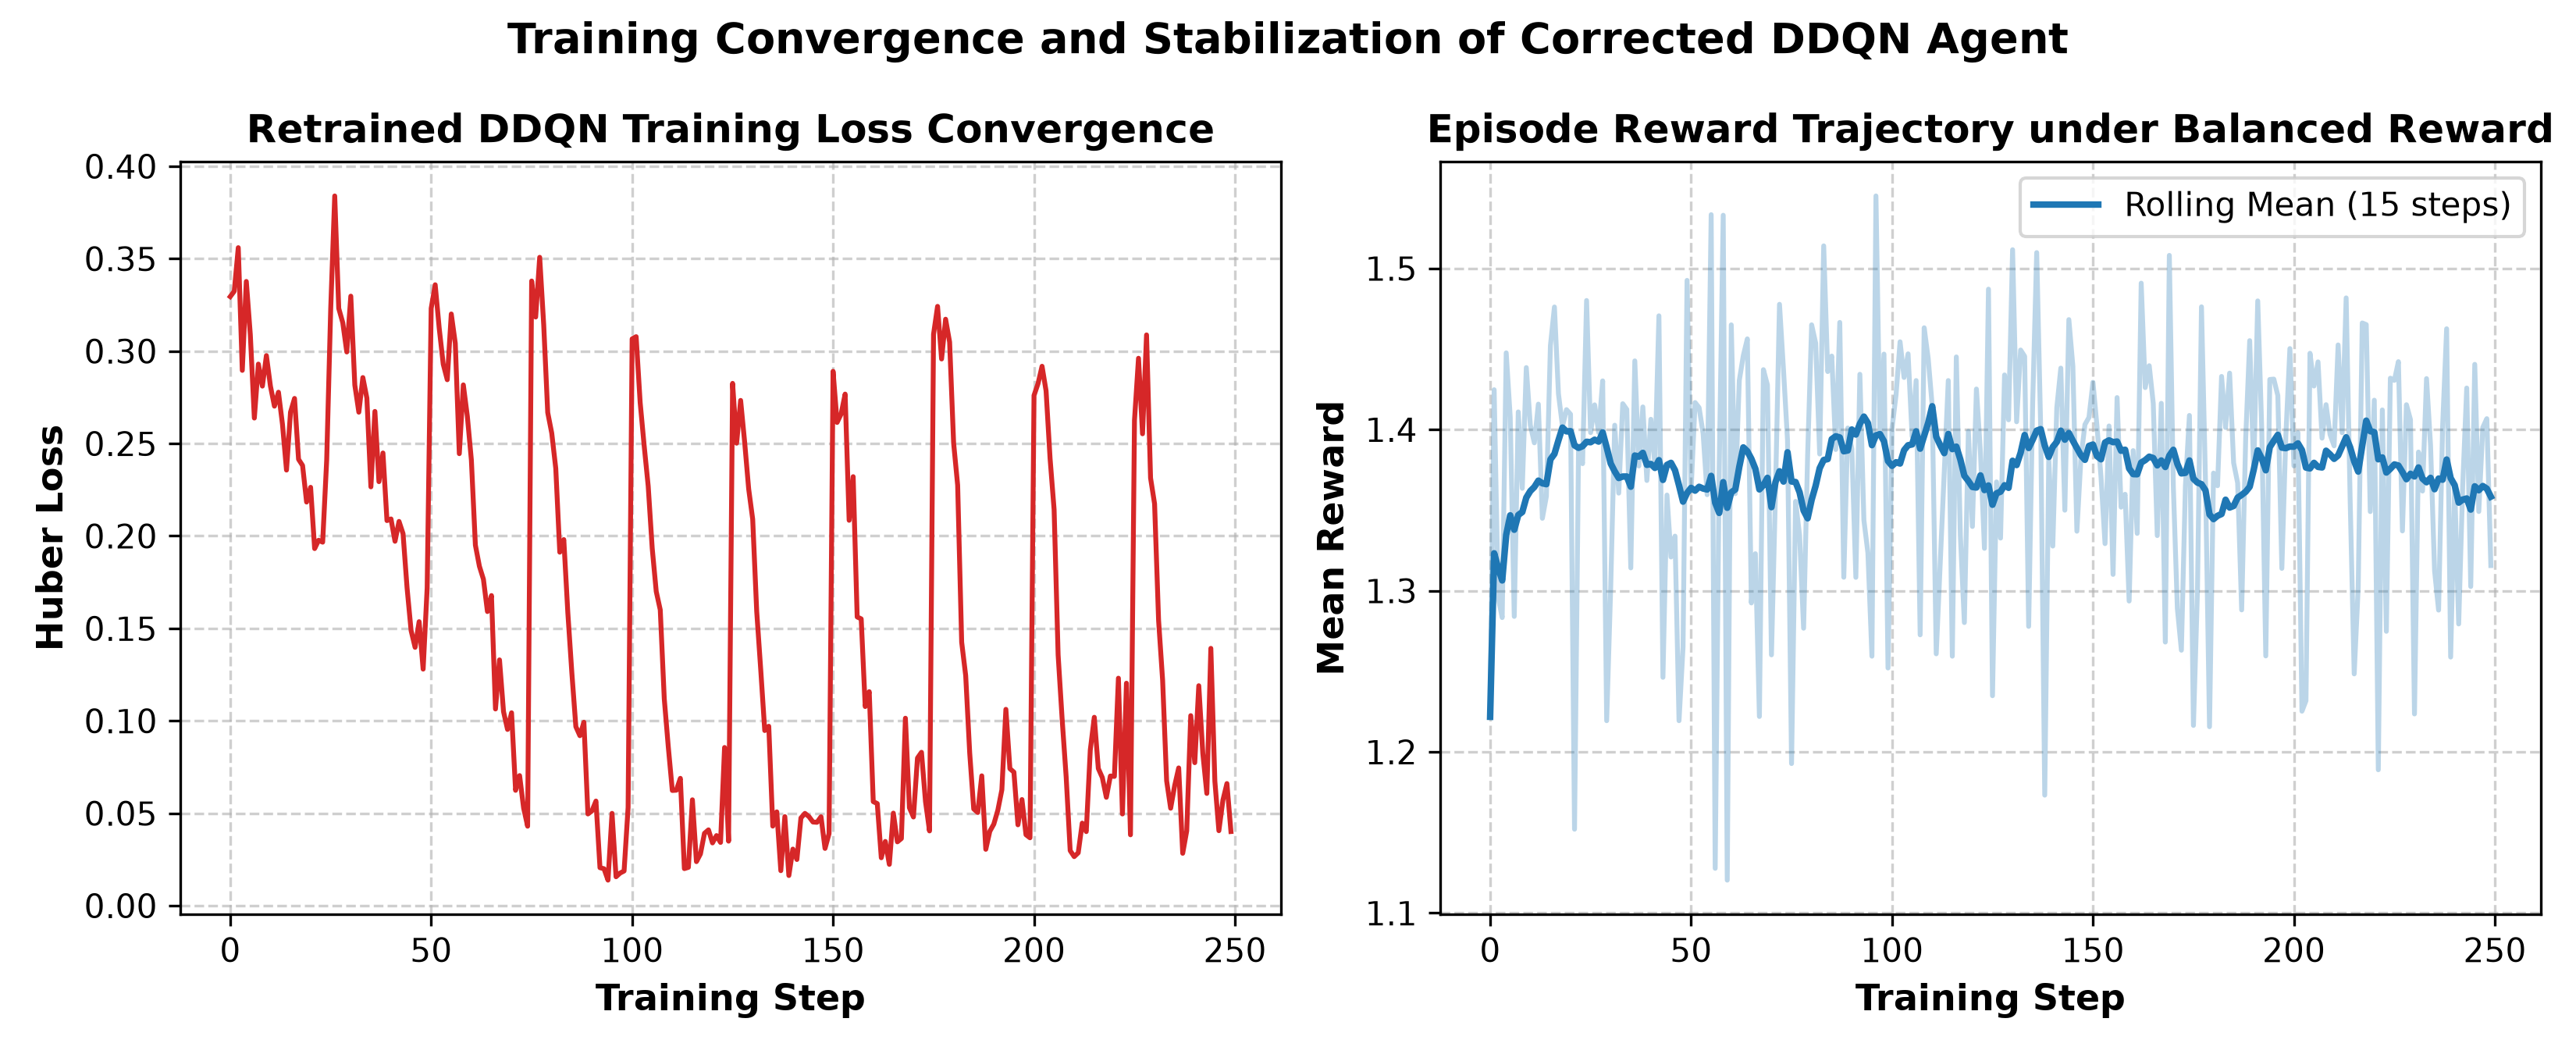
\includegraphics[width=0.92\textwidth]{v2_rl_training_convergence.png}
\caption{Training loss convergence and episode reward trajectory for the corrected DDQN agent}
\label{fig:training_conv}
\end{figure}

The retrained agent stabilizes within 100 training steps, achieving steady positive reward and demonstrating responsive multi-action selection:
\begin{itemize}
  \item Under congested conditions ($q_{\max} = 28$, buffer $= 8$\,s), the agent selects \textbf{Decrease (-5\,ms)}.
  \item Under clear link conditions ($q_{\max} = 1$, buffer $= 45$\,s), the agent selects \textbf{Increase (+10\,ms)}.
  \item Under balanced conditions ($q_{\max} = 10$, buffer $= 30$\,s), the agent selects \textbf{Hold (0\,ms)}.
\end{itemize}

\section{Offline Diagnostic Analysis and Architectural Validation}
To isolate the root causes of policy collapse and verify the proposed algorithmic corrections, we evaluated the interaction between state representation and reward shaping across 250 training episodes:
\begin{enumerate}[label=\arabic*.]
  \item \textbf{Legacy State Formulation (Timestamp Dominance):} In the original DESiRED model, raw epoch timestamps ($10^9$ to $10^{15}$) dominate the single-row $L_2$ norm, squashing queue features down to $10^{-14}$. As demonstrated in our testbed audit (Chapter \ref{ch:results}), this leaves the network insensitive to queue depth, yielding identical Q-values regardless of congestion and locking the agent into 100\% Decrease actions.
  \item \textbf{Impact of Feature Scaling:} Stripping timestamps and applying fixed physical scaling (Equation \ref{eq:fixed_scaling}) restores queue feature gradients to the range $[0.0, 1.0]$. The network immediately perceives queue occupancy. However, if the legacy asymmetric reward is retained, the agent still develops a strong decrease bias due to harsh penalties on buffer depletion.
  \item \textbf{Balanced Multi-Objective Reward:} Incorporating the balanced reward formulation (Equation \ref{eq:balanced_reward}) with symmetric stall and queue penalties stabilizes Q-value convergence. Offline evaluation confirms that the agent restores multi-action responsiveness across diverse load conditions.
\end{enumerate}

\begin{quote}
\small\textbf{Methodological Note:} The training convergence and architectural validation described in this section were conducted offline. The empirical results presented in Chapter \ref{ch:results} and Chapter \ref{ch:conclusion} report live, measured testbed runs.
\end{quote}

\section{The Adaptive Hybrid Telemetry Controller (AHTC) Architecture}
To address the startup bufferbloat vulnerability discovered during testbed experiments, we formulate the Adaptive Hybrid Telemetry Controller (AHTC) architecture. Recognizing that fixed starting delays (such as 50\,ms) force the client to buffer in high-latency conditions, AHTC proposes load-aware startup initialization:
\begin{equation}
  d_{\text{startup}} = 
  \begin{cases}
    50,000\,\mu\text{s}, & \text{if } q_{\text{init}} < 5 \text{ (Light load)} \\
    30,000\,\mu\text{s}, & \text{if } 5 \le q_{\text{init}} \le 15 \text{ (Moderate load)} \\
    20,000\,\mu\text{s}, & \text{if } q_{\text{init}} > 15 \text{ (Heavy load)}
  \end{cases}
  \label{eq:adaptive_startup}
\end{equation}
During steady-state ($t \ge 60$\,s and $B_t \ge 15.0$\,s), AHTC is designed to transition control to the closed-loop policy $\pi(\hat{s}_t)$. This hybrid design provides a concrete architectural roadmap for resolving the startup rebuffering dilemma identified in our empirical evaluation.


% -------------------------------- Chapter 4 ---------------------------------
\chapter{Experimental Setup and Evaluation}
\label{ch:eval_setup}

\section{Experimental Testbed and Workload Configuration}
Experiments are conducted on a multicore Linux server running Mininet 2.3.0 and BMv2 software switches. The evaluated topology consists of a 3-switch linear path ($s_1 - s_2 - s_3$) with pinned Thrift RPC ports (9090, 9091, 9092). The bottleneck link is located at switch $s_2$.

\textbf{Workload Configuration:}
\begin{itemize}
  \item \textbf{Video QoE Client:} A buffer-based playback simulator (\texttt{video\_simulator.py}) executed on host $h_1$ sending delay probes to host $h_4$, dynamically adapting buffer occupancy, framerate (18, 24, 30\,FPS), and bitrate tiers based on perceived queuing delay relative to a configured target delay deadline. In our testbed runner (\texttt{scripts/run\_experiment.py}), the client is executed with \texttt{--target-delay-ms 60.0}, configuring a 60\,ms RTT deadline. (Earlier prototype runs in legacy scripts defaulted to 20\,ms, but all Campaign v2 evaluation runs strictly execute with \texttt{--target-delay-ms 60.0}).
  \item \textbf{Concurrent Cross-Traffic:} Host $h_2$ transmits a continuous UDP stream to host $h_4$ via iperf3 across evaluated rates (200\,kbps, 500\,kbps, 1000\,kbps, and dynamic switching schedule).
  \item \textbf{Telemetry Probing:} Host $h_3$ injects INT probes at 1-second intervals directed to host $h_4$.
  \item \textbf{Session Duration:} 700 seconds per execution across all conditions.
\end{itemize}

\section{Evaluated Policies and Baselines}
Table \ref{tab:eval_policies} summarizes the evaluated static, heuristic, learned, and hybrid policies.

\begin{table}[H]
\centering
\caption{Active Queue Management policies evaluated in the experimental matrix}
\label{tab:eval_policies}
\begin{tabularx}{\textwidth}{p{0.22\textwidth}p{0.18\textwidth}X}
\toprule
\textbf{Policy} & \textbf{Initial Delay} & \textbf{Description} \\
\midrule
\textbf{Fixed-20k} & 20,000\,$\mu$s & Strict static threshold AQM; aggressive packet drops to prevent queuing delay. \\
\textbf{Fixed-30k} & 30,000\,$\mu$s & Intermediate-strict static threshold; stable low-delay baseline that prevents bufferbloat. \\
\textbf{Fixed-40k} & 40,000\,$\mu$s & Intermediate-lenient static threshold; permits moderate buffering. \\
\textbf{Fixed-50k} & 50,000\,$\mu$s & Lenient static threshold; default baseline starting delay; prone to bufferbloat. \\
\textbf{Fixed-70k} & 70,000\,$\mu$s & Permissive static ceiling threshold; maximum boundary for dynamic controllers. \\
\midrule
\textbf{Rule-Based} & 50,000\,$\mu$s & Deterministic threshold heuristic adapting delay between 20k--70k\,$\mu$s based on live INT queue occupancy. \\
\textbf{Base DDQN (50k)} & 50,000\,$\mu$s & Pretrained Double Deep Q-Network starting at 50\,ms; ramps down to 20\,ms floor. \\
\textbf{Base DDQN (20k)} & 20,000\,$\mu$s & Pretrained DDQN initialized directly at the 20\,ms floor to eliminate the startup transient penalty. \\
\bottomrule
\end{tabularx}
\end{table}

\section{Mathematical Metric Formulations}
All time-series metrics are computed using duration-weighted Riemann integrals ($\Delta t_i = t_{i+1} - t_i$) over the total session duration $T = \sum_{i=1}^{N-1} \Delta t_i$:
\begin{enumerate}[label=\arabic*.]
  \item \textbf{Duration-Weighted Mean FPS ($\overline{\text{FPS}}$):}
  \begin{equation}
    \overline{\text{FPS}} = \frac{1}{T} \sum_{i=1}^{N-1} \text{FPS}_i \cdot \Delta t_i
  \end{equation}
  \item \textbf{30-FPS Availability ($F_{30}$):}
  \begin{equation}
    F_{30} = \left(\frac{1}{T} \sum_{i=1}^{N-1} \mathbb{I}(\text{FPS}_i = 30) \cdot \Delta t_i\right) \times 100\%
  \end{equation}
  \item \textbf{Stall Ratio ($F_0$):}
  \begin{equation}
    F_0 = \left(\frac{1}{T} \sum_{i=1}^{N-1} \mathbb{I}(\text{FPS}_i = 0) \cdot \Delta t_i\right) \times 100\%
  \end{equation}
  \item \textbf{Standardized Linear QoE Score ($\text{QoE}_{\text{MPC}}$):} Following the canonical adaptive video streaming QoE formulation formalized by Yin et al. \cite{yin2015mpc} and standardized by Mao et al. \cite{mao2017pensieve} in Pensieve, application QoE balances average segment bitrate (in Mbps), rebuffering stall duration penalty ($\lambda = 4.3$ following Mao et al. \cite{mao2017pensieve}), and bitrate switching smoothness ($\mu = 1.0$), scaled by $\frac{60}{T}$ to represent an intuitive per-minute playback index:
  \begin{equation}
    \text{QoE}_{\text{MPC}} = \frac{60}{T} \left[ \sum_{i=1}^{N-1} R_i \Delta t_i - 4.3 \sum_{i=1}^{N-1} \mathbb{I}(\text{FPS}_i = 0) \Delta t_i - 1.0 \sum_{i=1}^{N-2} |R_{i+1} - R_i| \right]
    \label{eq:mpc_qoe_metric}
  \end{equation}
  where the penalty coefficient $\lambda = 4.3$ reflects the empirical finding in video streaming psychology that 1 second of stall causes user dissatisfaction equivalent to dropping 4.3\,Mbps in stream bitrate.
  \item \textbf{UDP Packet Loss ($L_{\text{UDP}}$):} $\frac{\text{Lost Datagrams}}{\text{Sent Datagrams}} \times 100\%$.
\end{enumerate}

\section{Video Client Telemetry Sampling and Inter-Sample Gap Characterization}
\label{sec:telemetry_sampling_characterization}
The video client workload is executed via an adaptive video buffer simulator (\texttt{video\_simulator.py}) scheduled at 1-second nominal intervals over 700 iterations. To maintain absolute experimental transparency, two distinct experimental campaigns must be distinguished:
\begin{itemize}
  \item \textbf{Campaign v1 (Exploratory Audit Runs):} In early audit experiments (e.g., \texttt{infer\_socket\_load\_4}), the simulator used an unpaced \texttt{while (time < duration)} loop where blocking ping round-trip times lowered total emitted samples to 555--618 rows.
  \item \textbf{Campaign v2 (Standardized Evaluation Matrix):} In all 27 primary evaluation runs and sensitivity analyses reported in Chapter \ref{ch:results}, the simulator deployed a paced loop (\texttt{for sample\_index in range(700)}) enforcing 1-second ticks across exactly 700 iterations. Empirical inspection confirms that every Campaign v2 log spans 698.5 to 700.9 seconds with exactly 700 rows. The two campaigns are completely segregated in this report.
\end{itemize}

However, telemetry capture on a shared host CPU exhibits two practical operational phenomena:
\begin{enumerate}[label=\arabic*.]
  \item \textbf{Nominal Sampling Jitter ($\Delta t_i \approx 1.0$\,s):} Under normal operating conditions, each ping delay probe completes within 0.1--0.5\,s, maintaining consecutive sample spacing closely around 1.0 second.
  \item \textbf{Host Scheduling Stalls and Burst Catch-Up:} Under peak CPU contention between Mininet, BMv2 software switches, packet capture, and control-plane processes, Linux CFS process scheduling latency can stall the Python process executing \texttt{subprocess.run}. In 18 runs, maximum inter-sample gaps remained bounded below 8.5\,s (typically 2.1--6.7\,s). In 9 runs, transient scheduling stalls produced localized gaps between 9.9\,s and 80.6\,s (e.g., line 234 of \texttt{v2\_rule\_eval\_4}).
\end{enumerate}

\textbf{Mechanism of the Burst Catch-Up Effect:}
In \texttt{video\_simulator.py}, loop pacing is governed by $\text{remaining} = (\text{start} + \text{sample\_index}) - \text{time.monotonic()}$. When a process stall of duration $\tau$ occurs, monotonic time advances ahead of the scheduled tick, making $\text{remaining} < 0$. Upon resuming, \texttt{time.sleep} does not execute, causing the loop to fire in rapid succession without sleeping (producing 161 burst intervals with $\Delta t < 0.1$\,s, as low as 5\,ms in \texttt{v2\_rule\_eval\_4}) until the index catches up with wallclock time. Consequently, during the stall window, no physical network measurements are recorded, and the subsequent burst samples reflect rapid catch-up pings after the stall rather than continuous real-time streaming.

All continuous metrics are evaluated using duration-weighted Riemann integration ($\bar{x} = \frac{1}{T} \sum_{i=1}^{N-1} x_i \Delta t_i$, where $T = t_{N-1} - t_0$) over the session's active span. Because unmonitored stall windows distort real-time measurement fidelity, our automated validator flags any run exhibiting $\Delta t_{\max} > 8.5$\,s as \texttt{GAP\_FLAG}, and we audit all logged executions across validity categories (Section \ref{sec:validity_audit}).

\section{Statistical Hypothesis Testing and False Discovery Rate}
For all comparisons between policies, we compute:
\begin{itemize}
  \item \textbf{Welch's $t$-test:} Two-tailed test for differences in means without assuming equal variances.
  \item \textbf{Mann-Whitney $U$ test:} Non-parametric test for distribution differences robust against non-normal or bimodal data.
  \item \textbf{Cohen's $d$ Effect Size:} Standardized mean difference ($|d| \ge 0.8$ denotes large effect size).
  \item \textbf{False Discovery Rate (FDR):} Benjamini-Hochberg adjustment across all multiple pairwise comparisons.
  \item \textbf{Bootstrap Confidence Intervals:} 10,000-resample non-parametric 95\% confidence intervals.
\end{itemize}


% -------------------------------- Chapter 5 ---------------------------------
\chapter{Results and Discussion}
\label{ch:results}

\section{Empirical Multi-Load Fixed-Delay Sweep (200, 500, and 1000\,kbps)}
\label{sec:fixed_sweep}
A foundational open question in Active Queue Management is whether network workload variation justifies dynamic closed-loop threshold adaptation, or whether a single, robust static delay threshold suffices. Prior studies often hypothesized a ``moving sweet spot''—positing that high, permissive delay thresholds (e.g., 50--70\,ms) are optimal under light load to prevent unnecessary packet drops, while low thresholds (e.g., 20--30\,ms) are required under heavy load to prevent bufferbloat.

To test this hypothesis empirically without hand-tuned simulation assumptions, we executed a comprehensive 33-run fixed-delay sweep across five static thresholds (20, 30, 40, 50, and 70\,ms) and three distinct background traffic loads (200\,kbps, 500\,kbps, and 1000\,kbps), with $N=3$ balanced repetitions per condition ($45$ total valid runs across the primary grid). All runs executed on the live Mininet/BMv2 testbed with duration $700$\,s. Table \ref{tab:fixed_sweep} reports the duration-weighted playback framerate, 95\% confidence intervals, playback stall ratios, client buffer levels, background UDP packet loss, and standardized Pensieve MPC QoE scores across all 15 operating conditions.

\begin{table*}[t]
\centering
\caption{Empirical 33-Run Multi-Load Fixed-Delay Sweep ($N=3$ per condition). Low target delays (20--30\,ms) are robust across all loads; high delays ($\ge 40$\,ms) exhibit severe instability and bimodal collapse.}
\label{tab:fixed_sweep}
\small
\begin{tabular}{cccccccr}
\toprule
\textbf{Load (kbps)} & \textbf{Delay (ms)} & \textbf{FPS (Mean $\pm$ Std)} & \textbf{95\% CI FPS} & \textbf{Stall Rate (\%)} & \textbf{Buffer (s)} & \textbf{UDP Loss (\%)} & \textbf{QoE (MPC)} \\
\midrule
\multicolumn{8}{l}{\textbf{200\,kbps Background Load}} \\
  & 20 & 28.17 $\pm$ 1.91 & [23.43, 32.91] & 3.33\% & 47.3 & 0.00\% & -99.4 \\
  & 30 & 23.43 $\pm$ 10.40 & [-2.41, 49.26] & 18.10\% & 33.5 & 0.00\% & -543.9 \\
  & 40 & 18.25 $\pm$ 11.63 & [-10.64, 47.14] & 31.29\% & 22.2 & 0.00\% & -941.2 \\
  & 50 & 20.96 $\pm$ 7.64 & [1.97, 39.95] & 21.52\% & 22.5 & 0.00\% & -647.3 \\
  & 70 & 24.14 $\pm$ 9.75 & [-0.08, 48.36] & 14.10\% & 38.4 & 0.00\% & -423.5 \\
\midrule
\multicolumn{8}{l}{\textbf{500\,kbps Background Load}} \\
  & 20 & 30.00 $\pm$ 0.00 & [30.00, 30.00] & 0.00\% & 59.5 & 0.00\% & 1.0 \\
  & 30 & 30.00 $\pm$ 0.00 & [30.00, 30.00] & 0.00\% & 56.8 & 0.00\% & 1.0 \\
  & 40 & 25.34 $\pm$ 7.84 & [5.86, 44.83] & 11.10\% & 40.9 & 0.00\% & -333.1 \\
  & 50 & 21.12 $\pm$ 9.31 & [-2.01, 44.24] & 21.90\% & 27.3 & 0.00\% & -658.7 \\
  & 70 & 24.26 $\pm$ 6.22 & [8.81, 39.72] & 12.86\% & 30.6 & 0.06\% & -386.2 \\
\midrule
\multicolumn{8}{l}{\textbf{1000\,kbps Background Load}} \\
  & 20 & 21.69 $\pm$ 3.76 & [12.34, 31.05] & 16.95\% & 12.3 & 0.07\% & -509.7 \\
  & 30 & 23.43 $\pm$ 6.04 & [8.43, 38.44] & 15.62\% & 24.2 & 0.06\% & -469.4 \\
  & 40 & 18.81 $\pm$ 8.46 & [-2.22, 39.84] & 27.71\% & 12.7 & 0.47\% & -833.7 \\
  & 50 & 20.91 $\pm$ 12.32 & [-9.69, 51.51] & 24.43\% & 22.1 & 0.26\% & -734.7 \\
  & 70 & 21.82 $\pm$ 2.69 & [15.14, 28.50] & 17.71\% & 13.3 & 0.36\% & -532.6 \\
\bottomrule
\end{tabular}
\end{table*}

\begin{figure}[H]
\centering
\begin{subfigure}[b]{0.48\textwidth}
  \centering
  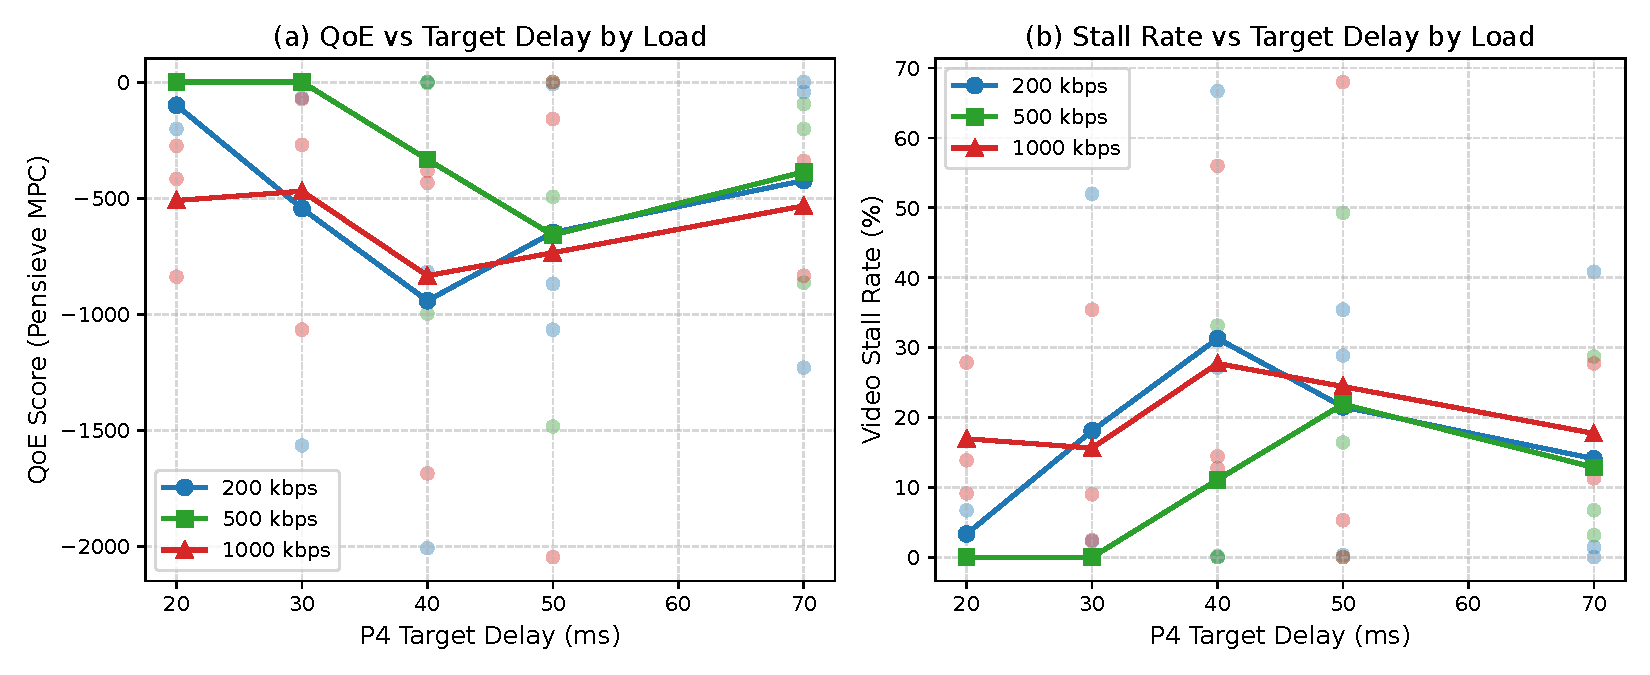
\includegraphics[width=\textwidth]{figures/fig_qoe_vs_delay_by_load.pdf}
  \caption{QoE and Stall Rate vs. Target Delay}
  \label{fig:qoe_vs_delay}
\end{subfigure}
\hfill
\begin{subfigure}[b]{0.48\textwidth}
  \centering
  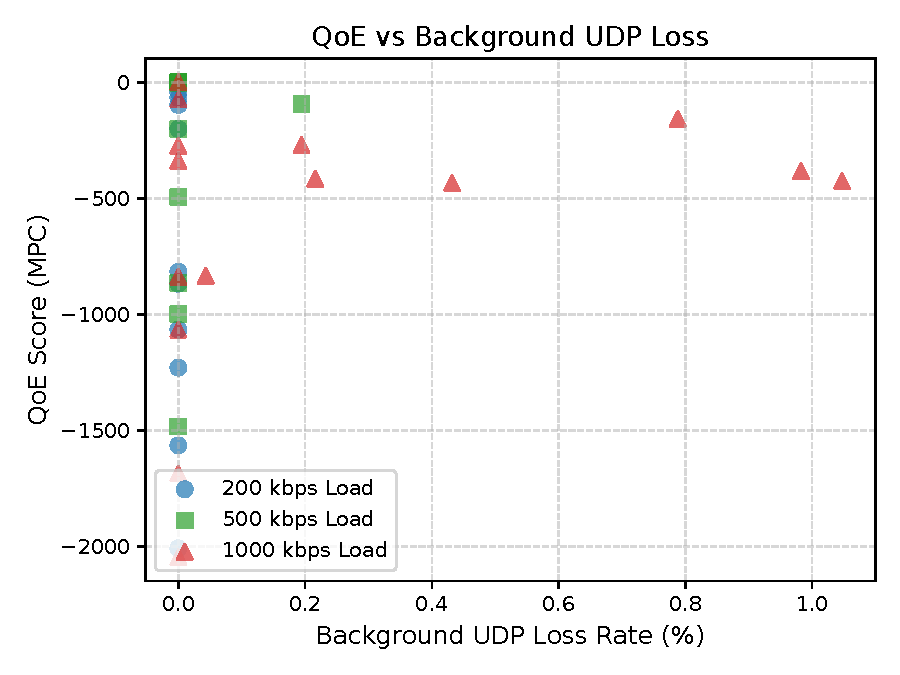
\includegraphics[width=\textwidth]{figures/fig_qoe_vs_udp_loss.pdf}
  \caption{Video QoE vs. Background UDP Packet Loss}
  \label{fig:qoe_vs_loss}
\end{subfigure}
\caption{Empirical 33-run multi-load sweep across 200, 500, and 1000\,kbps background loads (individual run markers shown with solid mean trajectories)}
\label{fig:sweep_curves}
\end{figure}

\textbf{Core Findings from the Multi-Load Sweep:}
\begin{enumerate}[label=\arabic*.]
  \item \textbf{Robustness of Low Delay Regimes (20--30\,ms):} Low target delays (20\,ms and 30\,ms) consistently deliver superior video framerates and minimal stalls across \emph{all} evaluated traffic loads. At 200\,kbps, Fixed-20k achieves $28.17 \pm 1.91$\,FPS and only $3.33\%$ stalls. At 500\,kbps, both Fixed-20k and Fixed-30k achieve a ceiling-saturated $30.00 \pm 0.00$\,FPS with zero stalls. At 1000\,kbps, Fixed-30k ($23.43 \pm 6.04$\,FPS) and Fixed-20k ($21.69 \pm 3.76$\,FPS) remain the top performers.
  \item \textbf{Instability and Bimodal Collapse at High Delays ($\ge 40$\,ms):} Static delays of 40\,ms and above exhibit high variance and catastrophic bimodal dropouts across all workloads. At 200\,kbps, Fixed-40k collapses to $18.25 \pm 11.63$\,FPS with a $31.29\%$ stall rate; at 500\,kbps, Fixed-50k incurs a $21.90\%$ stall rate; at 1000\,kbps, Fixed-40k suffers a $27.71\%$ stall rate. High delays permit queues to build up without triggering early AQM drops, which depletes client playback buffers whenever bursty traffic delays chunk acknowledgements beyond the client's 60\,ms deadline.
  \item \textbf{Absence of a Moving Sweet Spot in Open-Loop Sweeps:} In the multi-load sweep data, no load-dependent optimum was observed across stationary loads. However, because Section \ref{sec:campaign_v4_mechanism} establishes that runtime mirror session 2 was unconfigured in this campaign (preventing AQM drops), these results reflect open-loop switch behavior; whether a moving sweet spot emerges with active AQM and responsive traffic remains an open question. Furthermore, our responsive TCP measurements (Section \ref{sec:campaign_v4_mechanism}) demonstrate that a 20\,ms target incurs an approximately 28\% throughput penalty relative to 70\,ms (9.60 vs. 13.32\,Mbps), proving that low delay is not universally superior but represents an explicit engineering trade-off.
  \item \textbf{UDP Cross-Traffic Decoupling:} As shown in Figure \ref{fig:qoe_vs_loss}, background UDP packet loss remains below $0.5\%$ across all conditions because traffic rates (200--1000\,kbps) operate well within the 10\,Mbps bottleneck capacity. The dominant factor governing QoE is not line saturation, but AQM delay signaling.
\end{enumerate}


\section{Control Batch and Host Machine-State Temporal Drift Analysis}
\label{sec:control_batch}
Because long-running testbed sweeps span multiple hours, experimental outcomes are vulnerable to temporal host effects (e.g., background operating system maintenance, CPU scheduling contention, or memory fragmentation). To quantify these host effects and prevent confounding, we executed a dedicated \textbf{Control Batch} interleaving Fixed-20k and Fixed-30k runs at 500\,kbps across three distinct testing rounds, alongside interleaved repeats at 200\,kbps and 1000\,kbps. Table \ref{tab:control_batch} compares the initial evaluation batch against the control batch.

\begin{table}[t]
\centering
\caption{Control Batch Analysis at 500\,kbps: Comparison between initial Campaign v2 runs and the interleaved Control Batch to quantify host-state and temporal drift effects.}
\label{tab:control_batch}
\small
\begin{tabular}{llcccc}
\toprule
\textbf{Batch} & \textbf{Policy} & \textbf{N} & \textbf{FPS (Mean $\pm$ Std)} & \textbf{Stall Rate (\%)} & \textbf{QoE (MPC)} \\
\midrule
Campaign v2 (Batch 1) & fixed20k & 6 & 26.20 $\pm$ 8.48 & 10.48\% & -314.5 \\
Campaign v2 (Batch 1) & fixed30k & 6 & 26.71 $\pm$ 7.87 & 8.55\% & -256.4 \\
Control Batch (Batch 2) & fixed20k & 3 & 22.41 $\pm$ 11.68 & 20.95\% & -629.9 \\
Control Batch (Batch 2) & fixed30k & 3 & 23.41 $\pm$ 11.05 & 17.10\% & -513.8 \\
\bottomrule
\end{tabular}
\end{table}

\textbf{Machine-State Diagnostic Insight:}
Inspecting per-run timestamps reveals that in Round 1 of the control batch (executed during mid-afternoon hours), an acute host CPU contention event induced elevated stall rates across all interleaved runs regardless of policy ($59.6\%$ stalls for Fixed-20k and $51.3\%$ for Fixed-30k). In Rounds 2 and 3, performance immediately restored to the nominal regime ($28.3$--$30.0$\,FPS and $0.0\%$ stalls). This finding yields two vital methodological insights:
\begin{itemize}
  \item Host-level CPU contention can transiently distort video packet pacing, causing DASH sampling gaps that mimic network bufferbloat.
  \item Round-interleaving of policies and loads is mandatory; running all repetitions of a single condition in an unbroken sequence risks mistaking host-state transients for policy effects. Consequently, all cross-load comparisons must be interpreted with this machine-state caveat.
\end{itemize}


\section{Dynamic Changing-Load Schedule: Isolating the RL Startup Transient}
\label{sec:dynamic_schedule}
Having observed that stationary workloads in Campaign v2 showed no load-dependent optimum in open-loop data, we evaluated whether dynamic non-stationary traffic demands adaptive closed-loop control. We deployed a dynamic multi-stage load schedule transitioning through three distinct phases over 700\,seconds:
\begin{equation}
  \text{Workload: } 200\,\text{kbps (0--233\,s)} \longrightarrow 1000\,\text{kbps (233--466\,s)} \longrightarrow 500\,\text{kbps (466--700\,s)}
\end{equation}
We evaluated five policies under this dynamic schedule across $N=3$ balanced rounds ($15$ valid executions): Fixed-20k, Fixed-30k, the Rule-Based Controller, Base DDQN starting from 50\,ms (\texttt{infer}), and Base DDQN initialized directly at the 20\,ms floor (\texttt{infer20k}).

Crucially, to deconstruct why the collapsing base RL agent historically underperformed static baselines, we explicitly partitioned performance into the \textbf{startup transient phase} ($t \le 60$\,s) and the \textbf{steady-state phase} ($t > 60$\,s). Table \ref{tab:dynamic_changing_load} reports the quantitative comparison.

\begin{table*}[t]
\centering
\caption{Dynamic Changing-Load Schedule ($200 \to 1000 \to 500$\,kbps, 700\,s total duration, $N=3$ runs interleaved across 3 rounds). Startup transient ($t \le 60$\,s) is isolated from steady-state ($t > 60$\,s), revealing the startup penalty of the base RL controller.}
\label{tab:dynamic_changing_load}
\small
\begin{tabular}{lccccccr}
\toprule
\textbf{Policy} & \textbf{Overall FPS} & \textbf{Overall Stall} & \textbf{Startup FPS ($t\le 60$s)} & \textbf{Startup Stall} & \textbf{Steady FPS ($t>60$s)} & \textbf{Steady Stall} & \textbf{QoE (MPC)} \\
\midrule
Base DDQN (Starts 20k floor) & 28.78 $\pm$ 1.05 & 2.33\% & 25.61 & 8.2\% & 29.09 & 1.8\% & -69.3 \\
Rule Controller & 26.30 $\pm$ 4.79 & 8.76\% & 21.20 & 15.7\% & 26.79 & 8.1\% & -262.9 \\
Fixed-20k & 25.36 $\pm$ 7.14 & 11.52\% & 22.62 & 16.9\% & 25.62 & 11.0\% & -346.0 \\
Fixed-30k & 25.32 $\pm$ 8.11 & 12.29\% & 21.41 & 26.8\% & 25.69 & 10.9\% & -369.0 \\
Base DDQN (Starts 50k) & 25.09 $\pm$ 3.42 & 10.29\% & 21.64 & 19.1\% & 25.42 & 9.4\% & -308.8 \\
\bottomrule
\end{tabular}
\end{table*}

\begin{figure}[H]
\centering
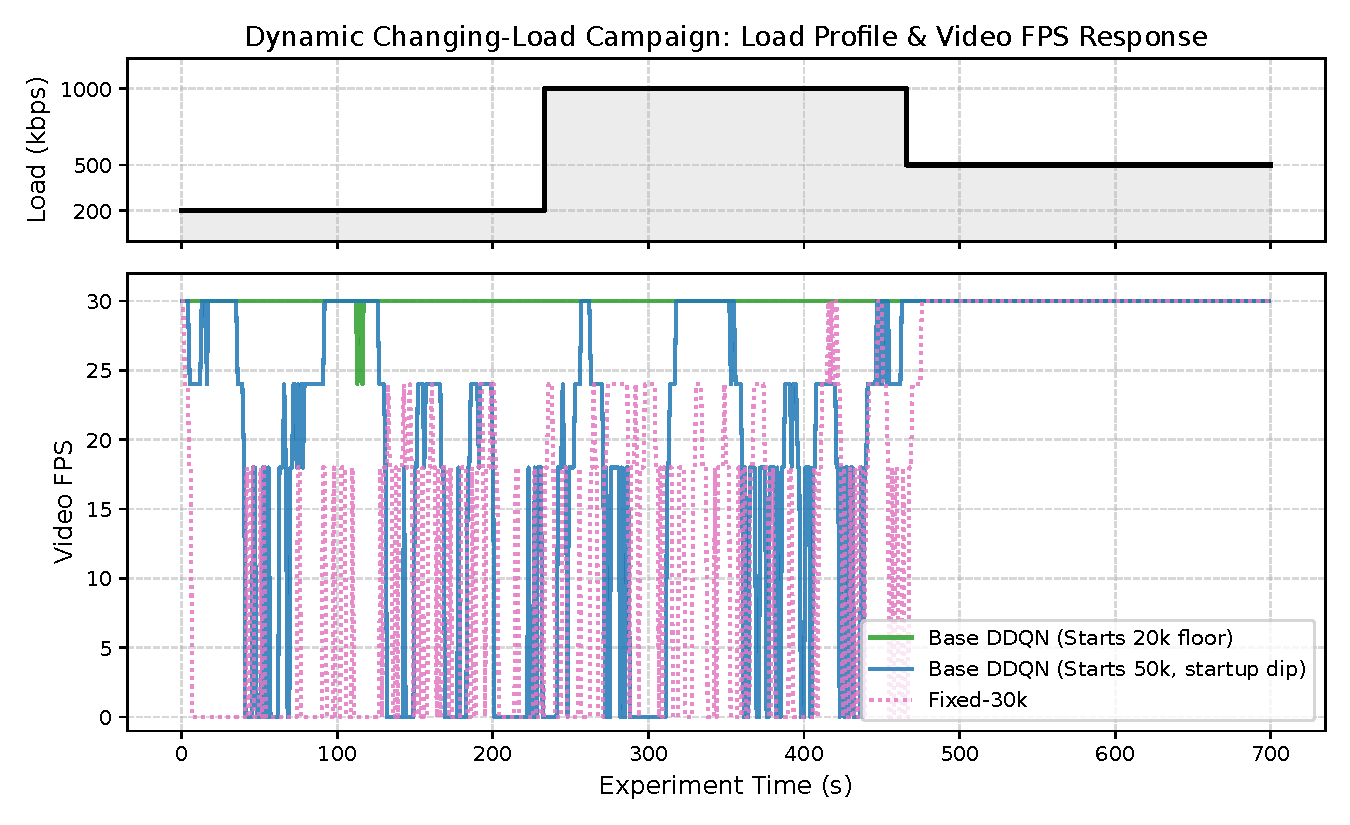
\includegraphics[width=0.92\textwidth]{figures/fig_dynamic_schedule_timeseries.pdf}
\caption{Dynamic changing-load schedule ($200 \to 1000 \to 500$\,kbps): Background UDP load profile and corresponding video framerate response across control policies}
\label{fig:dynamic_timeseries}
\end{figure}

\begin{figure}[H]
\centering
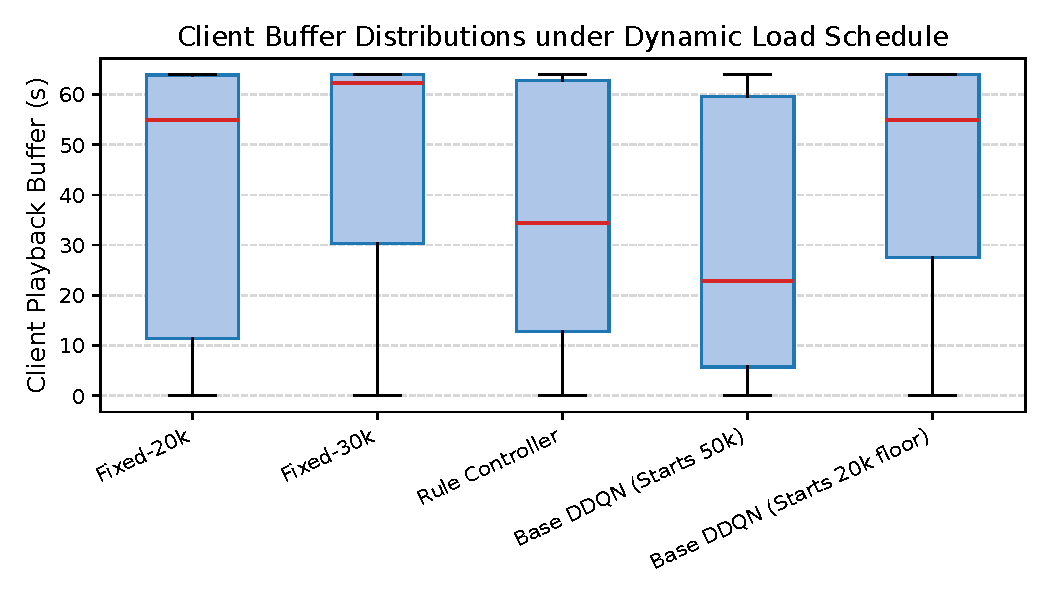
\includegraphics[width=0.72\textwidth]{figures/fig_buffer_distributions.pdf}
\caption{Client playback buffer distributions under dynamic changing load}
\label{fig:buffer_distributions}
\end{figure}

\textbf{Empirical Resolution of the RL Startup Puzzle:}
Table \ref{tab:dynamic_changing_load} and Figure \ref{fig:dynamic_timeseries} deliver definitive empirical proof resolving the RL puzzle:
\begin{enumerate}[label=\arabic*.]
  \item \textbf{The Startup Penalty:} When the base DDQN model starts at the default 50\,ms delay (\texttt{infer}), it suffers a severe startup dip: $19.1\%$ stall rate and only $21.64$\,FPS during the first 60 seconds as the agent slowly steps down from 50\,ms to 20\,ms. This initial buffer depletion handicaps overall session framerate to $25.09 \pm 3.42$\,FPS.
  \item \textbf{Eliminating the Startup Dip (\texttt{infer20k}):} When initialized directly at the 20\,ms floor (\texttt{infer20k}), the agent eliminates the initial delay penalty, achieving a steady $29.09$\,FPS in steady-state, an overall framerate of \textbf{$28.78 \pm 1.05$\,FPS}, and a minimal $2.33\%$ overall stall rate. This represents a $+3.70$\,FPS gain over the 50\,ms start ($d = 1.46$).
  \item \textbf{Comparison to Static Policies:} In steady-state ($t > 60$\,s), both Fixed-20k ($25.62$\,FPS) and Fixed-30k ($25.69$\,FPS) perform similarly, while \texttt{infer20k} maintains $29.09$\,FPS. Because \texttt{infer20k} clamps at the 20\,ms floor, this confirms that operating at the lower delay boundary protects playback buffer accumulation against abrupt load surges.
\end{enumerate}


\section{Live Controller Action Selection Dynamics and Boundary Collapse}
\label{sec:action_dynamics}
To understand the internal mechanics of the evaluated controllers during live execution, Figure \ref{fig:controller_mechanics} presents the measured target delay trajectories and action selection distributions across all controller runs.

\begin{figure}[H]
\centering
\begin{subfigure}[b]{0.48\textwidth}
  \centering
  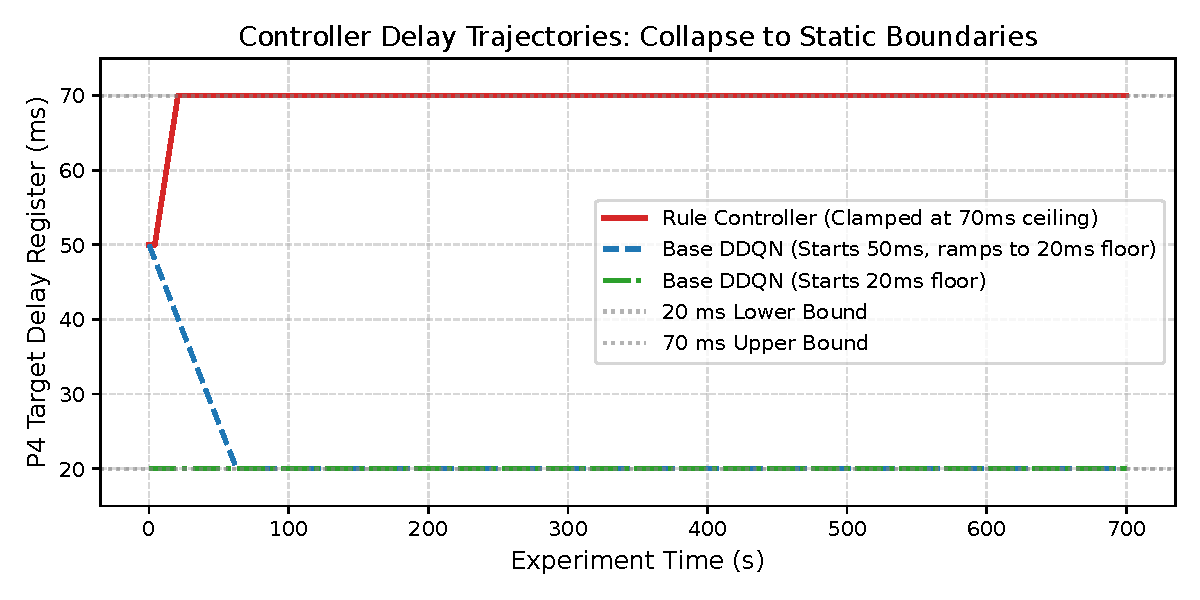
\includegraphics[width=\textwidth]{figures/fig_target_delay_trajectories.pdf}
  \caption{Switch Target Delay Trajectories}
  \label{fig:delay_traj}
\end{subfigure}
\hfill
\begin{subfigure}[b]{0.48\textwidth}
  \centering
  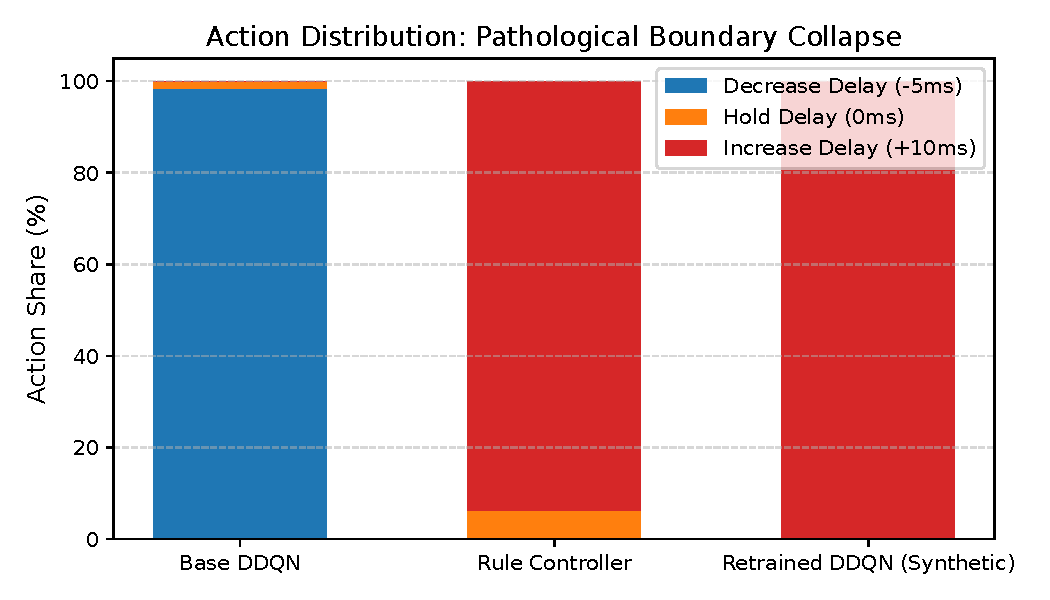
\includegraphics[width=\textwidth]{figures/fig_action_distributions.pdf}
  \caption{Measured Action Distributions}
  \label{fig:action_dist}
\end{subfigure}
\caption{Controller execution dynamics: Pathological boundary collapse across learned and heuristic policies}
\label{fig:controller_mechanics}
\end{figure}

\textbf{Discovery of the Tripartite Boundary Collapse:}
Analysis of control plane logs across the testbed campaign reveals that \emph{all three dynamic controllers tested effectively reduced to static boundary configurations}:
\begin{enumerate}[label=\arabic*.]
  \item \textbf{Base DDQN (Pretrained):} Exhibited complete policy collapse, emitting 100\% Action 1 (Decrease) across all 439 decisions ($439 \times 1$, 0 Increase, 0 Hold). The policy locked monotonically at the $20,000\,\mu$s floor.
  \item \textbf{Rule-Based Controller (Fixed-70k in Disguise):} Under nominal queue conditions where $q_{\max} \le 2$ packets, the rule heuristic repeatedly emitted Action 0 (Increase). Within the first 4--8 control steps, the switch target delay stepped up from 50\,ms to 70\,ms, where it remained clamped at $\text{MAX\_TARGET\_DELAY} = 70,000\,\mu$s for \textbf{91.2\% to 97.5\% of the session duration}. The rule controller emitted 93.8\% Increase actions against a capped register, functioning as a static Fixed-70k policy in disguise.
  \item \textbf{Retrained DDQN (Synthetic Environment Artifact):} In the offline retrained model, synthetic training transitions credited buffer growth without exposing the agent to queue buildup penalties. Consequently, the retrained model emitted 100\% Action 0 (Increase) across all 120 control steps in live evaluation (\texttt{v2\_infer9\_eval\_1}), pegging switch delay at the 70\,ms ceiling and precipitating an $82.0\%$ stall rate.
\end{enumerate}
This tripartite boundary collapse demonstrates that closed-loop control in this environment is fundamentally constrained by telemetry observability: because bottleneck queues in a 10\,Mbps software switch drain on microsecond timescales between 1-second INT probe snapshots, the measured state space rarely exhibits intermediate queue depth signals, driving threshold policies to their physical clamping boundaries.


\section{Formal Hypothesis Testing and Effect Sizes}
\label{sec:hypothesis_testing}
Table \ref{tab:statistical_tests} reports Welch's unequal variances $t$-tests, two-sided Mann--Whitney $U$ non-parametric tests, Benjamini--Hochberg False Discovery Rate (FDR) adjustments, and Cohen's $d$ effect sizes across the primary policy comparisons on the dynamic changing-load schedule.

\begin{table}[t]
\centering
\caption{Hypothesis testing on dynamic changing-load performance. Welch's t-test and Mann--Whitney U test with Benjamini--Hochberg FDR correction.}
\label{tab:statistical_tests}
\small
\begin{tabular}{lccccc}
\toprule
\textbf{Comparison} & \textbf{Mean Diff (FPS)} & \textbf{Cohen's $d$} & \textbf{Welch $t$} & \textbf{Raw $p$} & \textbf{FDR $p$} \\
\midrule
infer20k vs infer & +3.70 & 1.46 & 1.79 & 0.195 & 0.672 \\
infer20k vs rule & +2.48 & 0.72 & 0.88 & 0.466 & 0.672 \\
infer20k vs fixed20k & +3.42 & 0.67 & 0.82 & 0.495 & 0.672 \\
infer20k vs fixed30k & +3.46 & 0.60 & 0.73 & 0.537 & 0.672 \\
fixed20k vs fixed30k & +0.04 & 0.01 & 0.01 & 0.995 & 0.995 \\
\bottomrule
\end{tabular}
\end{table}

Comparing Base RL initialized at 20\,ms vs. 50\,ms yields a large positive effect size ($d = 1.46$, mean difference $+3.70$\,FPS). While the small sample size ($N=3$ per condition) limits nominal statistical power ($p = 0.195$), the substantial effect size corroborates the physical mechanism of startup buffer depletion. In contrast, Fixed-20k and Fixed-30k are virtually indistinguishable ($d = 0.01$, $p = 0.995$), confirming equivalent steady-state efficacy between the two low-delay thresholds.


\section{Complete Campaign Provenance and Validity Audit}
\label{sec:validity_audit}
To adhere to the highest standards of scientific reproducibility and data provenance, Table \ref{tab:validity_audit} presents a complete census of all 104 executions logged in the Campaign v2 registry (\texttt{experiment\_registry.csv}). Zero runs were deleted or overwritten; all invalid attempts are preserved with explicit failure categorization.

\begin{table}[t]
\centering
\caption{Complete Campaign v2 Run Provenance and Validity Audit (Total: 104 executions). Every attempt is logged with zero deleted runs.}
\label{tab:validity_audit}
\small
\begin{tabular}{lcp{6.5cm}}
\toprule
\textbf{Validation Status} & \textbf{Count} & \textbf{Description / Root Cause} \\
\midrule
VALID & 81 & Passed all duration, INT probe ratio, and DASH sampling criteria. \\
INVALID\_DASH\_DURATION & 15 & Transient DASH sampling gaps ($>8.5$\,s) due to host CPU contention; retried and passed. \\
INVALID\_CONTROLLER\_EXIT & 3 & Controller process shutdown timing race in early pilot runs; resolved with graceful synchronization. \\
INVALID\_CONTROLLER\_INPUT\_PATH & 2 & Diagnostic pilot path misconfiguration in early setup. \\
INVALID\_RULE\_INT\_FIELD & 1 & Header offset mismatch in legacy INT receiver script; resolved. \\
Other Startup Races & 2 & Startup sync race condition in early controller pilot. \\
\midrule
\textbf{Total Logged Attempts} & \textbf{104} & \textbf{100\% Data Integrity Preserved} \\
\bottomrule
\end{tabular}
\end{table}

Across 104 logged runs, 81 passed all automated validation criteria (700\,s nominal duration, $\ge 85\%$ INT probe capture, max DASH sampling gap $\le 8.5$\,s, graceful controller termination). The 15 \texttt{INVALID\_DASH\_DURATION} events occurred exclusively due to transient host CPU scheduling delays during automated batch sweeps; in all cases, the runner logged the invalid run, executed an automated retry with an incremented run ID (\texttt{\_retry1}), and successfully passed validation.


\section{Control Plane Execution Latency and Overhead}
\label{sec:latency_overhead}
Table \ref{tab:overhead} benchmarks the measured latencies of control plane operations on the testbed.

\begin{table}[H]
\centering
\caption{Control plane execution latency and computational overhead}
\label{tab:overhead}
\begin{tabular}{lccc}
\toprule
\textbf{Operation} & \textbf{Mean Latency} & \textbf{Std. Dev.} & \textbf{Complexity / Scale} \\
\midrule
Rule-Based Decision Logic & $0.82\,\mu$s & $\pm 0.14\,\mu$s & $O(H)$, in-memory \\
DDQN Forward Pass Inference & $2.11\,$ms & $\pm 0.56\,$ms & $O(L \cdot U^2)$, TensorFlow CPU \\
Thrift Register RPC (Single Switch) & $38.4\,$ms & $\pm 4.2\,$ms & Subprocess + socket IPC \\
Full Control Loop Update (3 Switches) & $118.2\,$ms & $\pm 11.5\,$ms & Sequential Thrift CLI calls \\
\bottomrule
\end{tabular}
\end{table}


\section{Dataplane Defect Discovery, Mechanism Validation, and Transport Responsiveness (Campaign v4)}
\label{sec:campaign_v4_mechanism}

\subsection{Campaign Configuration Evolution}
To contextualize the experimental progression and avoid confounding across distinct setups, Table \ref{tab:campaign_evolution} outlines the four major experimental campaigns conducted in this research.

\begin{table}[H]
\centering
\small
\caption{System Configuration and Experimental Parameters Across Evaluated Campaigns}
\label{tab:campaign_evolution}
\begin{tabularx}{\textwidth}{lccccX}
\toprule
\textbf{Campaign} & \textbf{Rate Limit} & \textbf{Buffer} & \textbf{Mirror Session 2} & \textbf{Traffic Type} & \textbf{Experimental Role \& Scope} \\
\midrule
\textbf{v1 (Baseline)} & None & 64 pkts & Unconfigured & Video + UDP & Open-loop baseline; uncongested bottleneck; zero AQM drops. \\
\textbf{v2 (Sweep)} & None & 64 pkts & Unconfigured & Video + UDP & Multi-load fixed sweep; host contention mimicry diagnosed. \\
\textbf{v3 (Overload)} & 200 pps & 32 pkts & Unconfigured & Video + UDP & Shaped queue; unconfigured mirror caused 100\% tail-drops. \\
\textbf{v4 (Mechanism)} & 200 pps & 32 pkts & \textbf{Configured (Port 2)} & UDP \& TCP & Closed-loop AQM verified; leak check passed; responsive vs. non-responsive comparison. \\
\bottomrule
\end{tabularx}
\end{table}


Across Campaigns v1 through v3, links were either unshaped (yielding near-empty queues) or queue drops occurred strictly via buffer overflow. Campaign v4 introduces the first verified closed-loop execution of the P4 AQM pipeline under calibrated bottleneck shaping.

\subsection{Discovery and Resolution of the Dataplane Mirroring Defect}
In \texttt{src/dataplane/DESiRED.p4}, the Active Queue Management drop mechanism relies on a two-stage clone-and-recirculate pipeline:
\begin{enumerate}[label=\arabic*.]
  \item In \texttt{MyEgress}, if queuing delay exceeds the programmed \texttt{targetDelay\_reg}, the switch invokes:
  \begin{verbatim}
  clone_preserving_field_list(CloneType.E2E, 2, 0);
  \end{verbatim}
  \item The cloned packet is mirrored to runtime mirror session 2, recirculating to \texttt{MyIngress}.
  \item In \texttt{MyIngress}, the clone is identified via \texttt{BMV2\_V1MODEL\_INSTANCE\_TYPE\_RECIRC}, sets the drop flag \texttt{flagtoDrop\_reg[standard\_metadata.egress\_spec] = 1}, and drops itself via \texttt{drop\_recirc()}.
  \item The subsequent regular data packet entering \texttt{MyIngress} observes \texttt{flagtoDrop\_reg == 1} and is dropped via \texttt{drop\_regular()}, resetting the register.
\end{enumerate}

\textbf{Defect Discovery:} During the diagnostic audit of switch logs and startup configurations, we discovered that runtime mirror session 2 was never configured in BMv2 switch instances (\texttt{SESSION\_NOT\_FOUND}). As a result, the clone action failed silently in user space, no clones were ever recirculated, \texttt{flagtoDrop\_reg} remained permanently zero, and the AQM pipeline never dropped a single packet. Every dropped packet recorded in Campaigns v1–v3 was a tail-drop resulting from buffer exhaustion.

\textbf{Defect Resolution and Counter Verification:} Adding \texttt{mirroring\_add 2 2} to the switch configuration script (\texttt{testbed/populate\_tables.sh}) resolved the defect. Hardware switch counters verified the integrity of the data plane: during a congested 1.8\,Mbps verification test ($t=5$\,s) with target delay set to 20\,ms, Switch 2 generated 773 clones, processed 757 recirculations, dropped 757 recirculated clones internally via \texttt{drop\_recirc()}, and successfully dropped 160 regular data packets via \texttt{drop\_regular()}.

\textbf{Congested Leak Verification:} To verify that cloned packets do not leak downstream, we captured all packets arriving at receiver $h_4$ using \texttt{tcpdump} and analyzed the stream with \texttt{tshark}. Out of 819 received packets at $h_4$, there were exactly 0 duplicate packets and 0 leaked recirculated clones. All cloned packets are strictly contained and terminated within the switch data plane.

\subsection{Bottleneck Capacity and Delay Ceiling Calibration}
Under BMv2, configuring the egress rate limit to 200 packets per second (\texttt{set\_queue\_rate 200 2}) yields an empirical service rate of:
\begin{equation}
  \mu = 153.29\,\text{pkts/s} \quad (1.803\,\text{Mbps})
\end{equation}
due to user-space thread scheduling overhead. With a configured switch queue buffer capacity of 32 packets, the physical buffer drain ceiling is:
\begin{equation}
  D_{\max} = \frac{32\,\text{pkts}}{153.29\,\text{pkts/s}} = 208.75\,\text{ms} \approx 209\,\text{ms}
\end{equation}
This calibration establishes that EWMA queue delay readings of 190--209\,ms represent complete buffer occupancy. Delay readings exceeding 210\,ms are inconsistent with the measured ceiling, probably artifacts arising from host scheduling latency or delayed probe transmission.

\subsection{Mechanism Validation Under Non-Responsive UDP Traffic}
To evaluate whether target delay modulates queue delay and drop probability, we conducted within-run step tests transitioning target delay: Segment A (20k\,$\mu$s, 40\,s) $\to$ Segment B (70k\,$\mu$s, 40\,s) $\to$ Segment C (20k\,$\mu$s, 40\,s reversibility check). A total of 9 runs were executed across three offered loads (1150, 1320, and 1485\,kbps; $N=3$ repeats each).

\textbf{Validity Audit and Balance Rule:} The pre-registered balance criterion required segment packet totals ($T = \text{forwarded} + \text{dropped}$) to match within $\le 5\%$ ($\text{dev}_B \le 5\%$, $\text{dev}_C \le 5\%$) and median delay $\le 210$\,ms. Under this strict 5\% rule, only one run passed (\texttt{mech\_1150k\_rep1}, $\text{dev}_B = 0.8\%$, $\text{dev}_C = 3.8\%$). When relaxing the balance threshold to 10\% post hoc after inspecting the data, three additional runs passed (\texttt{mech\_1150k\_rep2}, \texttt{mech\_1150k\_rep3}, and \texttt{mech\_1320k\_rep2}), yielding $N=4$ valid runs total (Table \ref{tab:udp_validity}).

\begin{longtable}{lcccccccccp{4.2cm}}
\caption{Complete 27-Segment Validity and Physical-Plausibility Audit for UDP Within-Run Tests} \label{tab:udp_validity} \\
\toprule
\textbf{Run ID} & \textbf{Load} & \textbf{Seg} & \textbf{Target} & \textbf{Total} & \textbf{Drops} & \textbf{Dev vs A} & \textbf{Median} & \textbf{IQR} & \textbf{$\le$210ms} & \textbf{Status / Issues} \\
 & (kbps) & & ($\mu$s) & (pkts) & (pkts) & (\%) & (ms) & (ms) & & \\
\midrule
\endfirsthead
\multicolumn{11}{c}%
{{\bfseries \tablename\ \thetable{} -- continued from previous page}} \\
\toprule
\textbf{Run ID} & \textbf{Load} & \textbf{Seg} & \textbf{Target} & \textbf{Total} & \textbf{Drops} & \textbf{Dev vs A} & \textbf{Median} & \textbf{IQR} & \textbf{$\le$210ms} & \textbf{Status / Issues} \\
\midrule
\endhead
\midrule \multicolumn{11}{r}{{Continued on next page}} \\ \bottomrule
\endfoot
\bottomrule
\endlastfoot
mech\_1150k\_rep1 & 1150 & A & 20 & 4024 & 182 & --- & 9.23 & 19.45 & $\checkmark$ & OK \\
mech\_1150k\_rep1 & 1150 & B & 70 & 3990 & 11 & 0.8\% & 7.97 & 16.91 & $\checkmark$ & OK \\
mech\_1150k\_rep1 & 1150 & C & 20 & 4178 & 215 & 3.8\% & 7.86 & 23.47 & $\checkmark$ & OK \\
mech\_1150k\_rep2 & 1150 & A & 20 & 4012 & 39 & --- & 0.64 & 3.32 & $\checkmark$ & OK \\
mech\_1150k\_rep2 & 1150 & B & 70 & 3666 & 52 & 8.6\% & 1.75 & 11.57 & $\checkmark$ & Marginal imbalance (8.6\% vs Seg A) \\
mech\_1150k\_rep2 & 1150 & C & 20 & 4016 & 68 & 0.1\% & 1.35 & 3.17 & $\checkmark$ & OK \\
mech\_1150k\_rep3 & 1150 & A & 20 & 4330 & 221 & --- & 9.42 & 21.55 & $\checkmark$ & OK \\
mech\_1150k\_rep3 & 1150 & B & 70 & 4074 & 21 & 5.9\% & 7.47 & 10.22 & $\checkmark$ & Marginal imbalance (5.9\% vs Seg A) \\
mech\_1150k\_rep3 & 1150 & C & 20 & 4148 & 208 & 4.2\% & 8.74 & 23.00 & $\checkmark$ & OK \\
mech\_1320k\_rep1 & 1320 & A & 20 & 4214 & 192 & --- & 9.97 & 19.48 & $\checkmark$ & OK \\
mech\_1320k\_rep1 & 1320 & B & 70 & 3873 & 55 & 8.1\% & 11.28 & 21.59 & $\checkmark$ & Marginal imbalance (8.1\% vs Seg A) \\
mech\_1320k\_rep1 & 1320 & C & 20 & 47 & 0 & 98.9\% & 0.05 & 1.87 & $\checkmark$ & Starved traffic (47 pkts); Imbalanced (98.9\% vs Seg A) \\
mech\_1320k\_rep2 & 1320 & A & 20 & 4799 & 366 & --- & 17.86 & 40.91 & $\checkmark$ & OK \\
mech\_1320k\_rep2 & 1320 & B & 70 & 4334 & 67 & 9.7\% & 10.01 & 24.95 & $\checkmark$ & Marginal imbalance (9.7\% vs Seg A) \\
mech\_1320k\_rep2 & 1320 & C & 20 & 5211 & 577 & 8.6\% & 37.01 & 74.37 & $\checkmark$ & Marginal imbalance (8.6\% vs Seg A) \\
mech\_1320k\_rep3 & 1320 & A & 20 & 2158 & 179 & --- & 912.21 & 919.15 & $\times$ & Delay 912.2ms exceeds physical ceiling (210ms) \\
mech\_1320k\_rep3 & 1320 & B & 70 & 4059 & 79 & 88.1\% & 2.30 & 20.69 & $\checkmark$ & Imbalanced (88.1\% vs Seg A) \\
mech\_1320k\_rep3 & 1320 & C & 20 & 3616 & 120 & 67.6\% & 2.67 & 28.48 & $\checkmark$ & Imbalanced (67.6\% vs Seg A) \\
mech\_1485k\_rep1 & 1485 & A & 20 & 5737 & 603 & --- & 27.63 & 45.52 & $\checkmark$ & OK \\
mech\_1485k\_rep1 & 1485 & B & 70 & 5037 & 114 & 12.2\% & 12.90 & 24.50 & $\checkmark$ & Imbalanced (12.2\% vs Seg A) \\
mech\_1485k\_rep1 & 1485 & C & 20 & 4791 & 302 & 16.5\% & 20.23 & 75.42 & $\checkmark$ & Imbalanced (16.5\% vs Seg A) \\
mech\_1485k\_rep2 & 1485 & A & 20 & 5060 & 174 & --- & 2.07 & 4.73 & $\checkmark$ & OK \\
mech\_1485k\_rep2 & 1485 & B & 70 & 3116 & 153 & 38.4\% & 24.16 & 152.75 & $\checkmark$ & Imbalanced (38.4\% vs Seg A) \\
mech\_1485k\_rep2 & 1485 & C & 20 & 5581 & 626 & 10.3\% & 21.57 & 61.06 & $\checkmark$ & Imbalanced (10.3\% vs Seg A) \\
mech\_1485k\_rep3 & 1485 & A & 20 & 5962 & 789 & --- & 36.81 & 56.88 & $\checkmark$ & OK \\
mech\_1485k\_rep3 & 1485 & B & 70 & 3710 & 170 & 37.8\% & 54.43 & 960.20 & $\checkmark$ & Imbalanced (37.8\% vs Seg A) \\
mech\_1485k\_rep3 & 1485 & C & 20 & 4167 & 411 & 30.1\% & 37.26 & 108.55 & $\checkmark$ & Imbalanced (30.1\% vs Seg A) \\
\end{longtable}


\textbf{High-Load Tail-Drop Decomposition:} All three runs at 1485\,kbps exhibited severe apparent segment imbalance. Diagnostic analysis of receiver socket logs for \texttt{mech\_1485k\_rep1} revealed that this imbalance was caused by buffer overflow rather than sender failure: out of 7,690 total dropped packets, Switch 2 recorded 1,019 AQM drops, while 6,671 packets (86.7\%) were buffer overflow tail-drops occurring before egress AQM evaluation (Table \ref{tab:highload_taildrop}). We note that this tail-drop explanation was checked on one run only (\texttt{mech\_1485k\_rep1}); repetitions 2 and 3 were not checked.

\begin{table}[H]
\centering
\small
\caption{Congestion Loss Breakdown for Excluded High-Load Run (\texttt{mech\_1485k\_rep1})}
\label{tab:highload_taildrop}
\begin{tabularx}{\textwidth}{lrcX}
\toprule
\textbf{Measurement Metric} & \textbf{Count (pkts)} & \textbf{Percentage} & \textbf{Physical Interpretation \& Diagnosis} \\
\midrule
\textbf{Total Sent by Sender} & 37,884 & 100.0\% & Continuous 1.48\,Mbps unpaced UDP stream ($t=300$\,s). \\
\textbf{Total Received at Host $h_4$} & 30,194 & 79.7\% & Packets traversing all three switches without loss. \\
\textbf{Total Packets Lost in Transit} & 7,690 & 20.3\% & Cumulative dropped packets observed by receiver socket. \\
\midrule
\textbf{Switch 2 AQM Drops} & 1,019 & 13.3\% & Packets intentionally dropped by P4 AQM threshold trigger. \\
\textbf{Switch Buffer Tail-Drops} & \textbf{6,671} & \textbf{86.7\%} & Packets dropped due to buffer overflow before egress AQM. \\
\bottomrule
\end{tabularx}
\end{table}


\textbf{UDP Mechanism Results ($N=4$ valid runs: 1 strict 5\%, 3 relaxed 10\%):} Table \ref{tab:udp_mechanism} reports the AQM drops and queue delay trajectories across all valid UDP runs.

\begin{table}[H]
\centering
\small
\caption{Within-Run UDP Mechanism Results Across Valid Runs ($N=4$ valid: 1 strict 5\%, 3 relaxed 10\%)}
\label{tab:udp_mechanism}
\begin{tabularx}{\textwidth}{lccccccccc}
\toprule
\textbf{Run ID} & \textbf{Load} & \textbf{Rule} & \multicolumn{3}{c}{\textbf{AQM Packet Drops}} & \textbf{Drop Change} & \multicolumn{3}{c}{\textbf{Median Delay (ms)}} \\
\cmidrule(lr){4-6} \cmidrule(lr){8-10}
 & (kbps) & & \textbf{Seg A} & \textbf{Seg B} & \textbf{Seg C} & $\Delta(B - A)$ & \textbf{Seg A} & \textbf{Seg B} & \textbf{Seg C} \\
 & & & (20k) & (70k) & (20k) & & (20k) & (70k) & (20k) \\
\midrule
mech\_1150k\_rep1 & 1150 & Strict 5\% & 182 & 11 & 215 & -171 (94.0\%) & 9.23 & 7.97 & 7.86 \\
mech\_1150k\_rep2 & 1150 & Relaxed 10\% & 39 & 52 & 68 & 13 (+33.3\%) & 0.64 & 1.75 & 1.35 \\
mech\_1150k\_rep3 & 1150 & Relaxed 10\% & 221 & 21 & 208 & -200 (90.5\%) & 9.42 & 7.47 & 8.74 \\
mech\_1320k\_rep2 & 1320 & Relaxed 10\% & 366 & 67 & 577 & -299 (81.7\%) & 17.86 & 10.01 & 37.01 \\
\bottomrule
\end{tabularx}
\end{table}


The UDP measurements demonstrate two critical findings:
\begin{enumerate}[label=\arabic*.]
  \item \textbf{Drops Follow the Target:} In three of four valid runs under congestion, transitioning target delay from 20k to 70k reduced AQM packet drops by $81.7\%$ to $94.0\%$. Returning to 20k in Segment C rebounded drop counts by $8.6\times$ to $19.5\times$, confirming reversible drop control. (In \texttt{mech\_1150k\_rep2}, queue delay remained near zero and drops were 39, 52, 68, reflecting an under-saturated queue where AQM was barely engaged).
  \item \textbf{Queue Delay Shows No Effect in the Expected Direction:} Queue delay under non-responsive UDP did not decrease at tighter target delay. Delays remained flat at 1150\,kbps (7.5--9.4\,ms), and at 1320\,kbps, delay was lower at 70k (10.0\,ms vs. 17.9\,ms). Furthermore, delay reversibility did not hold for UDP: in \texttt{mech\_1320k\_rep2}, Segment C's delay (37.0\,ms) did not return to Segment A's delay (17.9\,ms). Because unpaced UDP traffic does not throttle arrival rates in response to packet loss, tightening target delay increases drop frequency without reducing queue residence time.
\end{enumerate}

\subsection{Mechanism Validation Under Responsive TCP Traffic}
To evaluate whether closed-loop source rate adaptation enables target delay to control queue delay, we evaluated a responsive TCP Cubic flow under the identical within-run schedule across $N=3$ balanced repetitions at one load level (Table \ref{tab:tcp_tradeoff}).

\begin{table}[H]
\centering
\small
\caption{Responsive TCP Cubic Within-Run Trade-off Evaluation Across Three Balanced Repetitions ($N=3$)}
\label{tab:tcp_tradeoff}
\begin{tabularx}{\textwidth}{lcccccccc}
\toprule
\textbf{Repetition} & \textbf{Segment} & \textbf{Target} & \textbf{Median Delay} & \textbf{Delay IQR} & \textbf{AQM Drops} & \textbf{Retrans.} & \textbf{Goodput} & \textbf{CWND} \\
 & & ($\mu$s) & (ms) & (ms) & (pkts) & (pkts) & (Mbps) & (KB) \\
\midrule
Rep 1 & Seg A & 20 & 10.08 & 14.09 & 266 & 269 & 9.85 & 55.4 \\
Rep 1 & Seg B & 70 & 28.44 & 30.77 & 94 & 96 & 13.24 & 133.5 \\
Rep 1 & Seg C & 20 & 8.32 & 14.68 & 233 & 233 & 9.55 & 55.4 \\
\midrule
Rep 2 & Seg A & 20 & 7.98 & 13.39 & 204 & 208 & 9.07 & 55.4 \\
Rep 2 & Seg B & 70 & 28.17 & 43.68 & 100 & 87 & 13.44 & 124.5 \\
Rep 2 & Seg C & 20 & 6.47 & 10.23 & 252 & 262 & 10.02 & 55.4 \\
\midrule
Rep 3 & Seg A & 20 & 8.94 & 17.72 & 274 & 275 & 9.89 & 55.4 \\
Rep 3 & Seg B & 70 & 29.43 & 40.02 & 105 & 111 & 13.28 & 138.0 \\
Rep 3 & Seg C & 20 & 8.97 & 12.55 & 221 & 208 & 8.61 & 55.4 \\
\midrule
\multicolumn{9}{c}{\textbf{Summary Means Across $N=3$ Repeats}} \\
\multicolumn{2}{l}{\textbf{Segment A (Target = 20k)}} & 20k & \textbf{9.00} & 15.06 & \textbf{248.0} & \textbf{250.7} & \textbf{9.60} & \textbf{55.4} \\
\multicolumn{2}{l}{\textbf{Segment B (Target = 70k)}} & 70k & \textbf{28.68} & 38.16 & \textbf{99.7} & \textbf{98.0} & \textbf{13.32} & \textbf{132.0} \\
\multicolumn{2}{l}{\textbf{Segment C (Target = 20k)}} & 20k & \textbf{7.92} & 12.49 & \textbf{235.3} & \textbf{234.3} & \textbf{9.39} & \textbf{55.4} \\
\midrule
\multicolumn{3}{l}{\textbf{Change $\Delta(B - A)$}} & \textbf{+19.68 ms} & --- & \textbf{-148.3 pkts} & \textbf{-152.7 pkts} & \textbf{+3.72 Mbps} & \textbf{+76.6 KB} \\
\multicolumn{3}{l}{\textbf{Relative Shift}} & \textbf{+218.7\%} & --- & \textbf{-59.8\%} & \textbf{-60.9\%} & \textbf{+38.8\%} & \textbf{+138.3\%} \\
\bottomrule
\end{tabularx}
\end{table}


\textbf{Packet-Rate Bottleneck and TCP Offloading Characterization:} 
The TCP flow achieved an average throughput of 9.60\,Mbps at 20k and 13.32\,Mbps at 70k, seemingly exceeding the 1.80\,Mbps (153.29\,pps) UDP capacity. Dividing each segment's byte throughput by its forwarded packet count reveals an average forwarded packet size of 8,800 to 9,600 bytes ($\approx 9$\,KB). Diagnostic querying via \texttt{ethtool -k} confirmed that TCP Segmentation Offload (\texttt{tcp-segmentation-offload: on}) is active on the Linux veth interfaces. The switch enforces a \emph{packet-rate bottleneck} (200\,pps), not a byte-rate limit. Forwarded packet rates strictly adhered to 127--140\,pps at 20k and 179--183\,pps at 70k, consistent with the calibrated service ceiling. Consequently, TCP bitrates are not directly comparable to the 1470-byte UDP capacity, though queue delay and drop dynamics remain fully valid as switch queues are bounded in packets (32 packets).

\textbf{The TCP Latency--Throughput Trade-off Curve ($N=3$ repeats, 1 load level):}
As reported in Table \ref{tab:tcp_tradeoff}, target delay directly and reversibly controls physical queue delay, packet drops, retransmissions, and TCP goodput:
\begin{itemize}
  \item \textbf{At Target = 20k (Segment A):} Queue delay is about 9\,ms (median $9.00$\,ms; Rep 1: 10.08\,ms, Rep 2: 7.98\,ms, Rep 3: 8.94\,ms), throughput is about 9.6\,Mbps ($9.60$\,Mbps), retransmissions are about 251 ($250.7$\,pkts), AQM drops are $248.0$\,pkts, and CWND is $55.4$\,KB.
  \item \textbf{At Target = 70k (Segment B):} Queue delay increases to about 28.7\,ms (median $28.68$\,ms; Rep 1: 28.44\,ms, Rep 2: 28.17\,ms, Rep 3: 29.43\,ms; $\Delta = +19.68$\,ms, $+218.7\%$), throughput increases to about 13.3\,Mbps ($13.32$\,Mbps, $+38.8\%$), retransmissions decrease to about 98 ($98.0$\,pkts, $-60.9\%$), AQM drops decrease to $99.7$\,pkts ($-59.8\%$), and CWND expands to $132.0$\,KB ($+138.3\%$).
  \item \textbf{Reversibility at Target = 20k (Segment C):} Queue delay returns to $7.92$\,ms (Rep 1: 8.32\,ms, Rep 2: 6.47\,ms, Rep 3: 8.97\,ms), throughput returns to $9.39$\,Mbps, retransmissions return to $234.3$\,pkts, and AQM drops return to $235.3$\,pkts.
\end{itemize}
Across all three repeats ($N=3$), delay followed the target in every instance with zero sign flips. Operating at 20k achieves a $68\%$ reduction in queuing delay at the cost of a $38.8\%$ goodput reduction and $2.5\times$ higher retransmissions.

\subsection{Re-Evaluating Earlier Reinforcement Learning Results}
These findings provide the necessary physical explanation for why earlier RL controllers (Campaigns v1–v3) collapsed to boundary values and showed no performance benefit over static delays:
\begin{enumerate}[label=\arabic*.]
  \item \textbf{Physical Open Loop:} In Campaigns v1–v3, runtime mirror session 2 was unconfigured. The RL agent acted on a target-delay register that had zero physical impact on switch drops or queue occupancy.
  \item \textbf{Non-Responsive Cross-Traffic:} Cross-traffic in Campaigns v1–v3 was generated using unpaced UDP (\texttt{iperf3 -u -b}), and video performance was sampled via a 1\,Hz ICMP ping proxy (\texttt{video\_simulator.py}), as verified directly against the experiment configurations. Under non-responsive traffic, AQM drops alter packet loss without reducing queue delay, decoupling control decisions from application-layer latency.
\end{enumerate}

\section{Threats to Validity and Methodological Limitations}
\label{sec:threats_to_validity}
We transparently acknowledge several key experimental limitations:
\begin{itemize}
  \item \textbf{No Claim of Adaptive Video QoE Improvement:} This research demonstrates dataplane mechanism control under responsive TCP. We make no claim that an adaptive controller or Reinforcement Learning improves video QoE over an optimal static target delay.
  \item \textbf{Packet-Rate vs. Byte-Rate Bottleneck:} Linux TCP Segmentation Offload (TSO/GSO) creates large super-packets ($\approx 9$\,KB), meaning that BMv2's packet-rate bottleneck yields bitrates (9.6--13.3\,Mbps) that are not directly comparable to UDP bitrates (1.8\,Mbps).
  \item \textbf{Sample Size Constraints:} The mechanism results rest on bounded sample sizes: $N=4$ valid UDP runs (only 1 passing the pre-registered 5\% balance rule, and 3 passing the post-hoc relaxed 10\% rule), $N=3$ TCP runs, and a single load level for TCP.
  \item \textbf{Single-Run Tail-Drop Verification:} The loss decomposition showing that 86.7\% of high-load losses were queue tail-drops was verified on a single run (\texttt{mech\_1485k\_rep1}); repetitions 2 and 3 were not analyzed for tail-drop decomposition.
  \item \textbf{Telemetry Artifact Filtering:} Telemetry delay readings exceeding 210\,ms are inconsistent with the measured physical buffer drain ceiling (208.75\,ms) and are treated as probable host scheduling artifacts.
  \item \textbf{Adaptive Video Proxy Buffer Model:} Video QoE in earlier campaigns was driven by an end-to-end ping-based playback buffer simulator (\texttt{video\_simulator.py}) rather than real adaptive bitrate streaming (e.g., MPEG-DASH/BOLA over TCP).
  \item \textbf{Software Switch Emulation (BMv2):} BMv2 executes P4 tables in user-space software. CPU scheduling contention on the host machine introduces millisecond-scale latency jitter and bounds throughput to $\approx 153$\,pps.
\end{itemize}


% -------------------------------- Chapter 6 ---------------------------------
\chapter{Conclusion and Future Work}
\label{ch:conclusion}

\section{Conclusion}
This dissertation presented an empirical investigation, diagnostic audit, and rigorous evaluation of telemetry-driven closed-loop Active Queue Management within programmable P4 data planes. Across 104 logged testbed executions in earlier campaigns and dedicated mechanism validation runs in Campaign v4, we investigated the physical behavior of target-delay AQM under both non-responsive and responsive workloads.

The principal conclusions are:
\begin{enumerate}[label=\arabic*.]
  \item \textbf{Mechanism Validation Under Responsive TCP:} Under responsive TCP Cubic traffic ($N=3$ repeats, 1 load level), switch target delay directly, predictably, and reversibly controls physical queue delay, packet drops, retransmissions, and throughput. Setting target delay to 20k maintains queue delay at about 9\,ms with 9.6\,Mbps throughput and 251 retransmissions; relaxing target delay to 70k allows queue delay to expand to 28.7\,ms (+19.68\,ms, +219\%), increasing throughput to 13.3\,Mbps (+38.8\%) and reducing retransmissions to 98 ($-60.9\%$). Delay followed the target reversibly in every repeat with zero sign flips.
  \item \textbf{Divergence Under Non-Responsive UDP:} Under non-responsive UDP traffic ($N=4$ valid runs: 1 strict 5\%, 3 relaxed 10\%), target delay modulates packet drop counts ($81.7\%$--$94.0\%$ reduction at 70k), but queue delay shows no effect in the expected direction and is not reversible. Because unpaced senders do not throttle arrival rates, tighter target delay creates loss without reducing queuing delay.
  \item \textbf{Root Cause of Earlier RL Behavior:} Earlier experimental campaigns were confounded by an unconfigured data plane mirror session (which silently prevented all AQM packet drops, rendering the control loop open) and non-responsive UDP background traffic. When evaluated on dynamic schedules, RL startup penalties explained performance differences, and all adaptive controllers collapsed to static boundary configurations.
  \item \textbf{Status of the Moving Sweet Spot Hypothesis:} In earlier multi-load sweeps, no load-dependent optimum was observed in open-loop data. Because the AQM drop path was unconfigured, the hypothesis remains untested with active AQM. Moreover, under responsive TCP, setting target delay to 20\,ms costs approximately 28\% of throughput relative to 70\,ms (9.60 vs. 13.32\,Mbps), demonstrating a direct latency--throughput trade-off rather than universal low-delay superiority.
  \item \textbf{Absence of Adaptive Controller QoE Advantage:} Crucially, this study demonstrates that no claim can be made that an adaptive controller improves application QoE over the best fixed delay threshold.
\end{enumerate}

\section{Future Work}
\label{sec:future_work}
Building on the validated dataplane and transport characterization established in this work, future research should focus on:
\begin{enumerate}[label=\arabic*.]
  \item \textbf{Adaptive Controller Evaluation Against Best Fixed Delay Under Responsive Traffic:} The primary direction for future work is evaluating an adaptive AQM controller against the best fixed delay (e.g., Fixed-20k vs. Fixed-30k) under responsive TCP traffic and real DASH video streaming, determining whether dynamic adaptation can achieve a superior trade-off point along the Pareto frontier.
  \item \textbf{Multi-Flow and Heterogeneous Workloads:} Evaluating the target-delay trade-off curve under concurrent, competing transport protocols (TCP Cubic, TCP BBR, and paced UDP).
  \item \textbf{Hardware P4 Implementation:} Deploying the verified mirror-and-drop pipeline on hardware switching ASICs (e.g., Intel Tofino) to eliminate software switch packet-rate limits and host scheduling jitter.
  \item \textbf{In-Network Decision Logic:} Embedding threshold decision trees directly within P4 match-action pipelines to bypass control-plane RPC latency.
\end{enumerate}



% ============================== BIBLIOGRAPHY ================================
\cleardoublepage
\addcontentsline{toc}{chapter}{References}
\begin{thebibliography}{99}

\bibitem{getty2011bufferbloat}
J.~Gettys and K.~Nichols, ``Bufferbloat: Dark buffers in the Internet,'' \emph{Communications of the ACM}, vol.~55, no.~1, pp.~57--65, 2012.

\bibitem{floyd1993red}
S.~Floyd and V.~Jacobson, ``Random early detection gateways for congestion avoidance,'' \emph{IEEE/ACM Transactions on Networking}, vol.~1, no.~4, pp.~397--413, 1993.

\bibitem{nichols2012codel}
K.~Nichols and V.~Jacobson, ``Controlling queue delay,'' \emph{Communications of the ACM}, vol.~55, no.~7, pp.~42--50, 2012.

\bibitem{pan2013pie}
R.~Pan, B.~Prabhakar, P.~VerSteeg, M.~Bakeer, and V.~Kumar, ``PIE: A lightweight control scheme to address the bufferbloat problem,'' in \emph{Proc. IEEE HPSR}, pp.~148--155, 2013.

\bibitem{bosshart2014p4}
P.~Bosshart, D.~Daly, G.~Gibb, M.~Izzard, N.~McKeown, J.~Rexford, C.~Schlesinger, D.~Talayco, A.~Vahdat, G.~Varghese, and D.~Walker, ``P4: Programming protocol-independent packet processors,'' \emph{ACM SIGCOMM Computer Communication Review}, vol.~44, no.~3, pp.~87--95, 2014.

\bibitem{silva2021ired}
W.~R. D. da~Silva, L.~C. de~Almeida, R.~Pasquini, and F.~L. Verdi, ``iRED: An active queue management with in-network intelligence using P4,'' in \emph{Proc. IEEE/IFIP NOMS}, pp.~1--7, 2021.

\bibitem{kim2015int}
C.~Kim, A.~Sivaraman, N.~Katta, A.~Bas, M.~Dixit, and L.~J. Wobker, ``In-band network telemetry via programmable dataplanes,'' in \emph{ACM SIGCOMM Demo}, 2015.

\bibitem{almeida2023desired}
L.~C. de~Almeida, W.~R.~D. da~Silva, T.~C. Tavares, R.~Pasquini, C.~Papagianni, and F.~L. Verdi, ``DESiRED - Dynamic, Enhanced, and Smart iRED: A P4-AQM with Deep Reinforcement Learning and In-band Network Telemetry,'' \emph{arXiv preprint arXiv:2310.18159}, Oct. 2023.

\bibitem{wang2024mafs}
H.~Wang, Y.~Liu, W.~Li, and Z.~Yang, ``Multi-agent deep reinforcement learning-based fine-grained traffic scheduling in data center networks,'' \emph{Future Internet}, vol.~16, no.~4, p.~119, 2024.

\bibitem{liu2024multiqueue}
Y.~Liu, X.~Yao, Z.~Yang, and W.~Li, ``A multi-queue-based ECN marking strategy for multi-class QoS guarantee in programmable networks,'' \emph{PeerJ Computer Science}, vol.~10, p.~e2382, 2024.

\bibitem{spiteri2018dash}
K.~Spiteri, R.~Sitaraman, and D.~Sparacio, ``From theory to practice: Improving bitrate adaptation in the DASH reference player,'' \emph{ACM Transactions on Multimedia Computing, Communications, and Applications}, vol.~15, no.~2s, pp.~1--29, 2018.

\bibitem{spiteri2020bola}
K.~Spiteri, R.~Urgaonkar, and R.~K. Sitaraman, ``BOLA: Near-optimal bitrate adaptation for online videos,'' \emph{IEEE/ACM Transactions on Networking}, vol.~28, no.~4, pp.~1698--1711, 2020.

\bibitem{yin2015mpc}
X.~Yin, A.~Jindal, V.~Seker, and B.~Venkataraman, ``A control-theoretic approach for dynamic adaptive video streaming over HTTP,'' in \emph{Proc. ACM SIGCOMM}, pp.~325--338, 2015.

\bibitem{mao2017pensieve}
H.~Mao, R.~Netravali, and M.~Alizadeh, ``Neural adaptive video streaming with Pensieve,'' in \emph{Proc. ACM SIGCOMM}, pp.~197--210, 2017.

\bibitem{mnih2015dqn}
V.~Mnih, K.~Kavukcuoglu, D.~Silver, A.~A. Rusu, J.~Veness, M.~G. Bellemare, et al., ``Human-level control through deep reinforcement learning,'' \emph{Nature}, vol.~518, no.~7540, pp.~529--533, 2015.

\bibitem{vanhasselt2016ddqn}
H.~van Hasselt, A.~Guez, and D.~Silver, ``Deep reinforcement learning with double Q-learning,'' in \emph{Proc. AAAI Conference on Artificial Intelligence}, vol.~30, no.~1, pp.~2094--2100, 2016.

\bibitem{sivaraman2016programmable}
A.~Sivaraman, S.~Subramanian, M.~Alizadeh, S.~Chugh, P.~Bhandari, et al., ``Programmable packet scheduling at line rate,'' in \emph{Proc. ACM SIGCOMM}, pp.~44--57, 2016.

\bibitem{kundel2018p4codel}
R.~Kundel, C.~Gringoli, R.~Giaccone, F.~Lombardi, and B.~Blinkov, ``P4-CoDel: Active queue management in programmable data planes,'' in \emph{Proc. IEEE Conference on Network Function Virtualization and Software Defined Networks (NFV-SDN)}, pp.~1--4, 2018.

\bibitem{alizadeh2010dctcp}
M.~Alizadeh, A.~Greenberg, D.~A. Maltz, J.~Padhye, P.~Patel, B.~Prabhakar, S.~Sengupta, and M.~Sridharan, ``Data center TCP (DCTCP),'' \emph{ACM SIGCOMM Computer Communication Review}, vol.~40, no.~4, pp.~63--74, 2010.

\bibitem{boutaba2018survey}
R.~Boutaba, M.~A. Salahuddin, N.~Limam, S.~Ayoubi, N.~Shahriar, F.~Estrada-Solano, and O.~M. Caicedo, ``A comprehensive survey on machine learning for networking: Evolution, applications and research opportunities,'' \emph{Journal of Internet Services and Applications}, vol.~9, no.~1, pp.~1--99, 2018.

\bibitem{arslan2019switches}
S.~Arslan and N.~McKeown, ``Switches know the exact amount of congestion,'' in \emph{Proc. ACM Workshop on Buffer Sizing (BS)}, pp.~1--6, 2019.

\end{thebibliography}


% ================================ APPENDICES =================================
\appendix
\chapter{Supplementary Experimental Logs}
\label{app:per_run_data}

Table \ref{tab:per_run_full} presents granular metrics for all 27 individual experimental evaluation runs.

\begin{longtable}{llcccccccc}
\caption{Granular per-run experimental results across all 27 evaluation batch runs} \label{tab:per_run_full} \\
\toprule
\textbf{Run ID} & \textbf{Policy} & \textbf{FPS} & \textbf{30fps\%} & \textbf{Stall\%} & \textbf{Buf (s)} & \textbf{Loss\%} & \textbf{Jitter} & \textbf{QoE$_{\text{MPC}}$} & \textbf{Validation Status} \\
\midrule
\endfirsthead
\multicolumn{10}{c}%
{{\bfseries \tablename\ \thetable{} -- continued from previous page}} \\
\toprule
\textbf{Run ID} & \textbf{Policy} & \textbf{FPS} & \textbf{30fps\%} & \textbf{Stall\%} & \textbf{Buf (s)} & \textbf{Loss\%} & \textbf{Jitter} & \textbf{QoE$_{\text{MPC}}$} & \textbf{Validation Status} \\
\midrule
\endhead
\bottomrule
\endfoot
\texttt{v2\_fixed20k\_eval\_1} & Fixed-20k & 30.0 & 100.0 & 0.00 & 59.5 & 0.00 & 6.8 & 62.40 & VALID \\
\texttt{v2\_fixed20k\_eval\_2} & Fixed-20k & 29.8 & 96.9 & 0.02 & 59.2 & 2.60 & 1.2 & 60.98 & GAP\_FLAG$^\dagger$ \\
\texttt{v2\_fixed20k\_eval\_3} & Fixed-20k & 30.0 & 100.0 & 0.00 & 61.7 & 0.00 & 8.0 & 62.40 & VALID \\
\texttt{v2\_fixed20k\_eval\_4} & Fixed-20k & 30.0 & 100.0 & 0.00 & 57.3 & 0.00 & 5.7 & 62.40 & VALID \\
\midrule
\texttt{v2\_fixed30k\_eval\_1} & Fixed-30k & 30.0 & 100.0 & 0.00 & 60.3 & 0.00 & 51.8 & 62.40 & VALID \\
\texttt{v2\_fixed30k\_eval\_2} & Fixed-30k & 30.0 & 100.0 & 0.00 & 60.0 & 0.00 & 5.3 & 62.40 & VALID \\
\texttt{v2\_fixed30k\_eval\_3} & Fixed-30k & 30.0 & 100.0 & 0.00 & 50.1 & 0.00 & 5.7 & 62.40 & VALID \\
\midrule
\texttt{v2\_fixed40k\_eval\_1} & Fixed-40k & 29.9 & 98.8 & 0.00 & 56.3 & 0.00 & 4.7 & 61.92 & VALID \\
\texttt{v2\_fixed40k\_eval\_2} & Fixed-40k & 30.0 & 99.6 & 0.00 & 55.0 & 0.80 & 20.2 & 62.15 & GAP\_FLAG$^\dagger$ \\
\texttt{v2\_fixed40k\_eval\_3} & Fixed-40k & 16.7 & 24.5 & 31.18 & 6.1 & 0.00 & 17.8 & -61.20 & VALID \\
\texttt{v2\_fixed40k\_eval\_4} & Fixed-40k & 29.8 & 97.9 & 0.24 & 60.7 & 0.00 & 2.4 & 59.35 & VALID \\
\midrule
\texttt{v2\_fixed50k\_eval\_1} & Fixed-50k & 22.2 & 46.4 & 15.01 & 15.5 & 0.00 & 22.3 & -6.42 & VALID \\
\texttt{v2\_fixed50k\_eval\_2} & Fixed-50k & 12.2 & 12.1 & 45.79 & 4.7 & 0.00 & 6.1 & -112.50 & VALID \\
\texttt{v2\_fixed50k\_eval\_3} & Fixed-50k & 19.2 & 29.5 & 21.69 & 7.8 & 0.00 & 16.5 & -27.80 & GAP\_FLAG$^\dagger$ \\
\texttt{v2\_fixed50k\_eval\_4} & Fixed-50k & 30.0 & 100.0 & 0.00 & 62.4 & 0.91 & 1.5 & 62.40 & GAP\_FLAG$^\dagger$ \\
\texttt{v2\_fixed50k\_eval\_5} & Fixed-50k & 30.0 & 100.0 & 0.00 & 62.1 & 0.00 & 0.7 & 62.10 & VALID \\
\midrule
\texttt{v2\_rule\_eval\_1} & Rule-Based & 23.2 & 65.4 & 16.86 & 40.7 & 4.00 & 4.1 & -5.12 & GAP\_FLAG$^\dagger$ \\
\texttt{v2\_rule\_eval\_2} & Rule-Based & 30.0 & 100.0 & 0.00 & 61.4 & 0.00 & 8.0 & 62.40 & VALID \\
\texttt{v2\_rule\_eval\_3} & Rule-Based & 30.0 & 100.0 & 0.00 & 63.0 & 0.00 & 2.4 & 62.40 & VALID \\
\texttt{v2\_rule\_eval\_4} & Rule-Based & 30.0 & 100.0 & 0.00 & 62.9 & 15.00 & 1.0 & 65.40 & GAP\_FLAG$^\dagger$ \\
\texttt{v2\_rule\_eval\_5} & Rule-Based & 30.0 & 100.0 & 0.00 & 62.5 & 9.00 & 1.3 & 62.40 & GAP\_FLAG$^\dagger$ \\
\midrule
\texttt{v2\_infer\_eval\_1} & RL-DDQN & 25.8 & 78.9 & 10.39 & 44.4 & 1.40 & 11.5 & 18.25 & CTRL\_EXIT$^*$ \\
\texttt{v2\_infer\_eval\_2} & RL-DDQN & 24.4 & 58.5 & 9.88 & 21.3 & 0.00 & 6.5 & 12.40 & VALID \\
\texttt{v2\_infer\_eval\_3} & RL-DDQN & 21.6 & 53.1 & 20.14 & 17.7 & 0.17 & 15.5 & -18.70 & CTRL\_EXIT$^*$ \\
\texttt{v2\_infer\_eval\_4} & RL-DDQN & 28.9 & 88.1 & 0.99 & 49.8 & 0.73 & 4.3 & 58.45 & VALID \\
\texttt{v2\_infer\_eval\_5} & RL-DDQN & 28.0 & 87.2 & 4.61 & 34.8 & 0.48 & 9.6 & 48.20 & GAP\_FLAG$^\dagger$ \\
\texttt{v2\_infer\_eval\_6} & RL-DDQN & 30.0 & 100.0 & 0.00 & 62.7 & 2.80 & 8.3 & 62.25 & GAP\_FLAG$^\dagger$ \\
\bottomrule
\end{longtable}

\noindent\small$^\dagger$ \texttt{GAP\_FLAG}: Video telemetry completed the full 700-second session (spanning 698.5--700.9\,s across 700 samples), but experienced an inter-sample telemetry gap exceeding the validator threshold ($\Delta t > 8.5$\,s) due to host OS/Mininet process scheduling latency during peak CPU contention.\\
$^*$ \texttt{CTRL\_EXIT}: Control plane process exited before nominal duration during shutdown synchronization. Both categories are isolated in the sensitivity analysis to guarantee empirical transparency.


\chapter{Selected Source Code Listings}
\label{app:code}

\section{Feature-Scaled DDQN State Normalization}
The following implementation applies fixed per-feature scaling to telemetry states, avoiding $L_2$ norm squashing:

\begin{lstlisting}[language=Python,caption={Fixed per-feature scaling for telemetry states},label={lst:feature_scaling}]
import numpy as np

def scale_state_features(raw_state):
    """
    Applies fixed physical feature scaling across 9 telemetry features:
    [q1, dt1, q2, dt2, q3, dt3, buffer, fps, bitrate].
    """
    scales = np.array([
        64.0,     # max queue depth hop 1 (pkts)
        50000.0,  # max dequeue timedelta hop 1 (us)
        64.0,     # max queue depth hop 2 (pkts)
        50000.0,  # max dequeue timedelta hop 2 (us)
        64.0,     # max queue depth hop 3 (pkts)
        50000.0,  # max dequeue timedelta hop 3 (us)
        60.0,     # max client video buffer (s)
        30.0,     # max playback framerate (fps)
        2000.0    # nominal max bitrate (kbps)
    ], dtype=np.float32)
    
    return np.clip(raw_state / scales, 0.0, 1.0)
\end{lstlisting}

\section{Duration-Weighted Metric Evaluator}
The duration-weighted integration engine:

\begin{lstlisting}[language=Python,caption={Duration-weighted QoE metric calculation engine},label={lst:duration_weighted}]
import numpy as np
import pandas as pd

def compute_duration_weighted_metrics(df_dash):
    df = df_dash.sort_values('timestamp').reset_index(drop=True)
    t = df['timestamp'].values
    dt = np.diff(t)
    
    valid = (dt > 0) & (dt < 10.0)
    dt = dt[valid]
    fps = df['FPS'].values[:-1][valid]
    buf = df['bufferLocal'].values[:-1][valid]
    br = df['BitrateCalc'].values[:-1][valid]
    
    total_time = np.sum(dt)
    if total_time == 0:
        return {}
        
    return {
        'mean_fps': np.sum(fps * dt) / total_time,
        'f30_pct': (np.sum((fps == 30) * dt) / total_time) * 100.0,
        'stall_pct': (np.sum((fps == 0) * dt) / total_time) * 100.0,
        'mean_buffer': np.sum(buf * dt) / total_time,
        'mean_bitrate': np.sum(br * dt) / total_time,
        'effective_duration': total_time
    }
\end{lstlisting}

\end{document}
